% main.tex — Composed master document for reading the full paper
%
% Compile from the core-research-material/ directory:
%   pdflatex main.tex
%   biber main
%   pdflatex main.tex
%   pdflatex main.tex
%
% Uses the 'standalone' package so each section file keeps its own
% \documentclass / \begin{document} wrapper and remains independently
% compilable.  When \input'd here the preamble is silently stripped.
%
% Missing image assets (add 'draft' to \documentclass options to get
% placeholder boxes instead of errors):
%   - cpu-gpu.svg              (sec2.2/2.2.1)
%   - *.png benchmark graphs   (sec3/3.3.1=TSP and sec3/3.2.1=XOR)

\documentclass[a4paper,14pt]{extarticle}
% All images now available — draft mode removed

% Pre-pass babel options before styles.sty loads it with only [english]
\PassOptionsToPackage{ukrainian,english}{babel}

\usepackage{standalone}        % strips preamble from \input'd standalone files
\usepackage{styles}            % project style package (biblatex, geometry, …)

% Additional packages for the composed document
\usepackage[T2A,T1]{fontenc}   % Cyrillic support for appendix pages
%\usepackage{svg}              % SVG figures (sec 2.2.1) — disabled until svg assets exist
\usepackage{pdflscape}         % landscape pages (Appendix A)
\usepackage{indentfirst}       % indent first paragraph after section headings

% Add each \litSubsubsection to the table of contents (no forced page break)
\let\origLitSubsubsection\litSubsubsection
\renewcommand{\litSubsubsection}[1]{%
  \origLitSubsubsection{#1}%
  \addcontentsline{toc}{subsubsection}{#1}%
}


% Bibliography resource (must be in preamble, not \AtBeginDocument)
\addbibresource{sources.bib}

\usepackage{array}             % \newcolumntype, \arraybackslash
\DeclareUnicodeCharacter{200B}{}  % ignore zero-width spaces (pasted from web)
% Column types used in Appendix A
\newcolumntype{L}[1]{>{\raggedright\arraybackslash}p{#1}}
\newcolumntype{C}[1]{>{\centering\arraybackslash}p{#1}}

\begin{document}

% ===== Title Page =====
\thispagestyle{empty}
% ---- begin title-page-eng.tex ----

\begin{titlepage}
\thispagestyle{empty}
\begin{center}
    Ministry of Education and Science of Ukraine\\[0.3cm]
    \textbf{National University of ``Kyiv-Mohyla Academy''}\\[0.3cm]
    Department of Computer Science of the Faculty of Informatics\\[1cm]

    
\includegraphics[width=4cm]{diagrams/title/naukma_logo.png}\\[1cm]

    \textbf{\large Optimization of Genetic Algorithm Computations through CUDA Parallel Processing}\\[0.3cm]

    Text part of the course paper in the specialty\\
    ``Computer Science'' -- 122\\[2cm]
\end{center}

\begin{flushright}
\begin{minipage}{0.5\textwidth}
    \raggedleft
    \textbf{Thesis Supervisor:}\\
    Senior Lecturer\\
    Sergii Medvid\\[0.3cm]
    \underline{\hspace{4cm}} (Signature)\\[0.3cm]
    ``\underline{\hspace{0.3cm}24\hspace{0.3cm}}'' \underline{\hspace{0.5cm}March\hspace{0.5cm}} 2026\\[0.3cm]
    \textbf{Done by Student:}\\
    Anastasiia Aleksieienko\\[0.3cm]
    \underline{\hspace{4cm}} (Signature)\\[0.3cm]
    ``\underline{\hspace{0.3cm}24\hspace{0.3cm}}'' \underline{\hspace{0.5cm}March\hspace{0.5cm}} 2026
\end{minipage}
\end{flushright}

\vfill
\begin{center}
    Kyiv, 2026
\end{center}
\end{titlepage}

% ---- end title-page-eng.tex ----
\newpage

% ===== Table of Contents =====
\tableofcontents
\newpage

% ===== Annotation (Ukrainian) =====
\selectlanguage{ukrainian}
\phantomsection
\addcontentsline{toc}{section}{Анотація}
% ---- begin annotation-ua.tex ----

\section*{Анотація}

\textbf{Алексєєнко~А.\,Д.} Оптимізація обчислень генетичних алгоритмів через паралельну обробку за допомогою CUDA. - Курсова робота. Національний університет <<Києво-Могилянська академія>>, факультет інформатики, кафедра інформатики. - Київ, 2026.

\bigskip
У роботі досліджується прискорення генетичних алгоритмів (ГА) через паралелізацію на GPU з використанням CUDA та Python-нативних ядер, JIT-компільованих бібліотекою Numba. Розроблено CUDA-ядра для основних операторів ГА - обчислення пристосованості, селекції, схрещування та мутації - та проведено порівняння з CPU-реалізаціями на задачах навчання XOR-перцептрона і комівояжера (TSP).

GPU-реалізації перевершують CPU при популяції понад 100 особин, досягаючи прискорення від 1,15$\times$ до 14,56$\times$ на NVIDIA RTX~2050. Усі відмінності статистично значущі ($p < 0{,}05$, Cohen's $d > 0{,}8$). Домінуючим вузьким місцем є передача даних між хостом і пристроєм, що вказує на можливість подальшого прискорення за рахунок GPU-резидентних еволюційних циклів. Кодову базу реорганізовано у публічно доступну Python-бібліотеку для розробки ГА із GPU-прискоренням.

\bigskip
\textbf{Ключові слова:} генетичні алгоритми, CUDA, паралелізація на GPU, Numba, оптимізація продуктивності, задача комівояжера, навчання нейронних мереж, Python, паралельні обчислення.

% ---- end annotation-ua.tex ----
\selectlanguage{english}
\newpage

% ===== Abstract (English) =====
\phantomsection
\addcontentsline{toc}{section}{Abstract}
% ---- begin annotation-eng.tex ----

\section*{Abstract}

\textbf{Aleksieienko~A.\,D.} Optimization of Genetic Algorithm Computations through CUDA Parallel Processing. - Course paper. National University of ``Kyiv-Mohyla Academy'', Faculty of Informatics, Department of Computer Science. - Kyiv, 2026.

\bigskip
This paper investigates the acceleration of genetic algorithms (GAs) through CUDA-based GPU parallelization using Python-native Numba JIT-compiled kernels. Custom kernels for fitness evaluation, selection, crossover, and mutation were benchmarked against CPU implementations on XOR perceptron training and the Traveling Salesman Problem.

GPU implementations outperform CPU baselines for populations exceeding 100 individuals, achieving speedups of 1.15$\times$ to 14.56$\times$ on an NVIDIA RTX~2050. All differences are statistically significant ($p < 0.05$, Cohen's $d > 0.8$). The dominant bottleneck is host-device data transfer, indicating further gains are achievable with fully GPU-resident evolutionary loops. The codebase was refactored into a publicly available Python library for GPU-accelerated GA development.

\bigskip
\textbf{Keywords:} genetic algorithms, CUDA, GPU parallelization, Numba, performance optimization, traveling salesman problem, neural network training, Python, parallel computing.

% ---- end annotation-eng.tex ----
\newpage

% ===== SECTION 1: INTRODUCTION =====
\section{Introduction}
% ---- begin introduction.tex ----


    \geometry{
        left=25mm,
        right=15mm,
        top=20mm,
        bottom=20mm
    }

    \setstretch{1.5}


    This course paper investigates the acceleration of genetic algorithms through CUDA-based GPU parallelization, covering both performance analysis and the development of reusable implementation components.

    \bigskip\textbf{Hypothesis.} The application of CUDA technology to parallelize computations in genetic algorithms 
    will enable significant acceleration of key operations: fitness function evaluation, 
    selection, crossover, and mutation - compared to sequential implementation on the CPU. 
    It is expected that parallelization efficiency will increase with population
    size and computational complexity of the fitness function, subject to the theoretical limits imposed by Amdahl's Law and data transfer overhead.

    \bigskip Parallel processing of large populations on the GPU is expected to improve the quality of
    solutions found, because it allows operation with significantly larger population sizes without
    a proportional increase in overall algorithm execution time. This opens up new
    possibilities for solving complex optimization problems in acceptable timeframes.

    \bigskip\textbf{Object of the Research.} Genetic algorithms represent the general domain of the research paper, serving as black-box optimization material.

    \bigskip\textbf{Subject of the Research.} Parallelization strategies and speedups achieved through CUDA form the specific focus, targeting custom kernel development for selection, crossover, mutation, and fitness evaluation on GPU.
    ​

    \bigskip\textbf{Research Gap.} A comparative analysis of publication volumes on Semantic Scholar\footnote{Semantic Scholar Academic Graph API v1. Endpoint: \texttt{GET .../graph/v1/paper/\allowbreak search?\allowbreak query=\{Q\}\&limit=1} (base URL: \texttt{api.semanticscholar.org}). The \texttt{total} field in the JSON response gives the match count; \texttt{\&year=2020-2025} was appended for five-year filtering. All queries: October~2025. Verification in March~2026: control returned \texttt{total:\,286918} (all-time) and \texttt{total:\,109069} (5-year), confirming proportionality with the original data.} (accessed October 2025) shows that GPU-accelerated genetic algorithm optimization is substantially less studied than established optimization domains. Table~\ref{tab:ss-gap} summarizes the result counts.

    \begin{table}[h]
    \centering
    \caption{Semantic Scholar publication counts by query (October 2025).}
    \label{tab:ss-gap}
    \small
    \begin{tabular}{p{0.55\textwidth}rrr}
    \hline
    \textbf{Query} & \textbf{All-time} & \textbf{5-year} & \textbf{Ratio}\textsuperscript{*} \\
    \hline
    databases clustering optimization (control) & 243{,}000 & 94{,}500 & 1$\times$ \\
    CUDA parallel processing genetic algorithms & 8{,}800 & 1{,}380 & 28$\times$ \\
    MapReduce parallel processing genetic algorithms optimization & 7{,}530 & 1{,}150 & 32$\times$ \\
    OpenCL parallel processing genetic algorithms & 6{,}250 & 946 & 39$\times$ \\
    \hline
    \multicolumn{4}{l}{\textsuperscript{*}Ratio = control all-time / query all-time, rounded.}
    \end{tabular}
    \end{table}

    Within this space, the majority of GPU implementations use native C/C++ CUDA kernels or high-level framework abstractions (EvoJAX, EvoTorch, EvoX). Python-native CUDA kernel development via Numba, despite NVIDIA's investment in a Python CUDA SDK, appears rarely in the evolutionary computation literature. This gap motivates an investigation into whether Python-native GPU kernel development can achieve competitive speedups while retaining the prototyping speed and accessibility advantages that Python offers over lower-level CUDA C/C++ workflows.

    \bigskip\textbf{Structure of the Paper.} Section~2 provides the theoretical background: a literature review of GPU-accelerated genetic algorithms (Section~2.1) and an overview of CUDA architecture with kernel design principles (Section~2.2). Section~3 presents the experimental methodology, benchmark configurations, and results for two test problems: XOR perceptron training (Section~3.2) and the Traveling Salesman Problem (Section~3.3), followed by a cross-benchmark analysis (Section~3.4). Section~4 describes the reusable GPU-accelerated GA library developed from the experimental code and validates its results against the original benchmarks. Section~5 summarizes the findings and outlines directions for future work.

% ---- end introduction.tex ----
\newpage

% ===== SECTION 2: THEORETICAL BACKGROUND =====
\section{Theoretical Background}

\subsection{GPU-GA Literature Review}

% ---- begin sec2.1-literature-review/2.1.1-ga-parallelization-potential.tex ----


\litSubsubsection{2.1.1 Genetic Algorithms Parallelization Potential}

Genetic algorithms (GAs) are metaheuristic optimization techniques inspired by natural selection, which simulate evolutionary processes through key operations: fitness evaluation, selection, crossover, and mutation. GAs are stochastic global search methods that combine two strategies: exploiting better solutions and exploring the search space~\cite{cheng2020parallel}. A GA maintains a population of candidate solutions (individuals), each encoded as a chromosome, and iteratively evolves them over generations. GAs belong to the class of black-box optimization methods where only objective function evaluations are required - no gradient information or problem-specific knowledge is needed~\cite{katoch2021review}. The concept originates from John Henry Holland's work at the University of Michigan~\cite{holland1975adaptation}, whose ``original goal was not to design algorithms to solve specific problems, but rather to formally study the phenomenon of adaptation as it occurs in nature''~\cite{mitchell1998introduction}.

\parahead{Applications and Problem Domains.}
GAs are effective for solving NP-hard problems such as the Traveling Salesman Problem (TSP), Vehicle Routing Problem (VRP), job-shop scheduling, and multi-objective optimization~\cite{goldberg1989genetic,katoch2021review}. They avoid local optima traps that complicate gradient-based methods and are suited for vast, discontinuous search spaces.

\parahead{Core Operations of Genetic Algorithms.}
The GA lifecycle comprises four operations:
\gaop{Fitness Evaluation} computes an objective function value for each individual independently - typically the main computational bottleneck.
\gaop{Selection} chooses parents probabilistically based on fitness (e.g., tournament, roulette wheel).
\gaop{Crossover} combines parent chromosomes to produce offspring (e.g., single-point, uniform).
\gaop{Mutation} introduces random changes to maintain diversity (e.g., bit-flip, swap).

Each generation, $n$ offspring are produced through selection, crossover ($P_c$), and mutation ($P_m$), then replace the current population~\cite{katoch2021review}. Figure~\ref{fig:ga-lifecycle} illustrates this generational loop.

\begin{figure}[H]
\centering
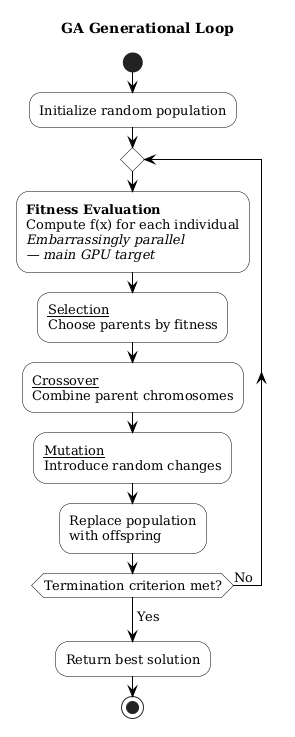
\includegraphics[width=0.45\textwidth]{diagrams/sec2/ga-lifecycle.png}
\caption{GA generational loop. Fitness evaluation is the primary GPU acceleration target due to its embarrassingly parallel nature.}
\label{fig:ga-lifecycle}
\end{figure}

\subsubsection*{Black-Box Optimization Nature and Parallelization Potential}

GAs are black-box optimizers: they evaluate solutions solely through fitness function calls, requiring no gradient computation or analytical models~\cite{katoch2021review}. ``The GA does not require derivative information or any other auxiliary knowledge about the function being optimized''~\cite{mitchell1998introduction}. In formal terms, the objective function is treated as an opaque oracle returning $f(\vect{x})$ given input $\vect{x}$, without revealing gradients or analytical form~\cite{audet2017derivative,nocedal2006numerical}.

This black-box property directly enables parallelization: since fitness evaluation has no inter-individual dependencies, each individual can be evaluated in complete isolation. This transforms population-wide fitness evaluation into an embarrassingly parallel workload, the ideal case for GPU acceleration where thousands of threads execute identical computations on different individuals~\cite{cheng2020parallel}. As Cheng and Gen note, ``on GPU architecture, you can run it with more than hundreds of thousands of massive threads simultaneously''~\cite{cheng2020parallel}.

Fitness evaluation dominates sequential GA execution time: ``the bottleneck of the GAs is the fitness evaluation task''~\cite{salami2002fitness}, and can consume the majority of total computation time for complex fitness functions such as neural network training~\cite{salami2002fitness}.

% ---- end sec2.1-literature-review/2.1.1-ga-parallelization-potential.tex ----
% ---- begin sec2.1-literature-review/2.1.2-cuda-model-suitability.tex ----


\litSubsubsection{2.1.2 CUDA Model Suitability for GA-Specific Computations}

\textbf{CUDA Model Suitability for GA-Specific Computations.} Compute Unified Device Architecture - ``CUDA is a parallel computing platform and programming model developed by NVIDIA that enables dramatic increases in computing performance by harnessing the power of the GPU''~\cite{nvidia2023cuda}. CUDA organizes computation into kernels executed by lightweight threads arranged in blocks and grids, with access to a hierarchical memory system (global, shared, constant, and texture memories). This architecture is well suited to data-parallel problems where the same operation is applied independently across large sets of data - a pattern that matches the population-based structure of GAs, where fitness evaluation and variation operators are applied repeatedly across individuals. The CUDA platform exposes GPU architectural features directly to programmers, enabling fine-grained control over thread execution to fully exploit GPU computing power~\cite{cheng2020parallel}.

\textbf{Python-CUDA Integration for GA Development.} The primary CUDA API uses C, but Python interfaces exist: CuPy provides NumPy-compatible GPU arrays backed by cuBLAS and cuFFT~\cite{cupy_docs}; Numba provides a JIT compiler that generates CUDA kernels directly from Python via the \texttt{@cuda.jit} decorator~\cite{numba_cuda}. These tools allow GA practitioners to implement operations in Python and delegate numeric workload to CUDA kernels on the GPU. ``Numba exposes the CUDA programming model, just like in CUDA C/C++, but using pure python syntax, so that programmers can create custom, tuned parallel kernels without leaving the comforts and advantages of Python behind.''\cite{harris2017numba}

\textbf{Benefits and Drawbacks of Python for CUDA GA Development.} Python is chosen for CUDA development in this paper to balance performance with rapid prototyping and accessibility. CuPy compiles custom kernels at runtime using NVRTC (NVIDIA Runtime Compilation), producing PTX that the driver compiles to device code, with results cached for reuse~\cite{cupy_docs}. Numba's JIT achieves performance close to native CUDA: ``CUDA Python Mandelbrot code runs nearly 1700 times faster than the pure Python version''~\cite{harris2017numba}. Python's concise syntax and ecosystem make it effective for disseminating GPU-accelerated GA techniques beyond systems programming specialists.

First, Python's interpreter adds host-side overhead to every GPU call; for small inputs the launch overhead can exceed the computation itself~\cite{carpentries_gpu}. Second, the Python-CUDA stack depends on multiple native libraries whose versions must align: CuPy requires a matched CUDA toolkit wheel~\cite{cupy_install}, and Numba requires both the toolkit and a compatible driver~\cite{numba_cuda}. Third, Python's GIL limits multi-core CPU orchestration of multiple GPUs, as it ``prevents multiple threads from executing Python code at the same time''~\cite{pep703}. These drawbacks are mitigated by focusing on large, compute-bound GA workloads with most computation on the device.

% ---- end sec2.1-literature-review/2.1.2-cuda-model-suitability.tex ----
% ---- begin sec2.1-literature-review/2.1.3-prior-studies.tex ----


\litSubsubsection{2.1.3 Prior GPU--GA Studies on GA Core Operations Optimization}

This subsection reviews relevant studies to identify patterns in GPU-accelerated GA computing. The review also examines the Python libraries and tools used.

\textbf{Study on Parallel Hybrid Genetic Algorithm and Machine Learning on GPU and Applications to Railway Scheduling.} Cheng and Gen~\cite{cheng2020parallel} parallelized a hybrid multi-objective GA applied to railway scheduling problems (ARL, BTS, and Japanese high-speed rail). The implementation offloaded differential evolution mutation, k-means clustering, and fitness evaluation to GPUs, which was necessary for maintaining practical computation times. The parallel implementation preserved solution quality while improving efficiency.

\textbf{GPU-Accelerated NSGA-II for Crystallization via Numba CUDA.} Rangavajhala et al.\ apply GPU-parallelized NSGA-II to crystallization process optimization, with the entire pipeline implemented using Numba CUDA kernels, achieving a $122\times$ speedup over the CPU baseline~\cite{rangavajhala2024accelerating}.

\textbf{GPU-Accelerated Stack-Based Genetic Programming: Sathia et al.} Candidate expressions are represented as prefix lists evaluated using fixed-length stacks in GPU memory. Benchmarked on an NVIDIA DGX-A100, the implementation achieves $119\times$ and $40\times$ speedups over gplearn on synthetic and large-scale datasets respectively~\cite{sathia2021accelerating}. The algorithm has been integrated into cuML, NVIDIA's scikit-learn-compatible GPU library~\cite{sathia2021accelerating}.

\textbf{EvoGP: GPU-Accelerated Tree-Based Genetic Programming.} Wu et al.\ present EvoGP, a GPU-accelerated framework for tree-based genetic programming that achieves up to $304\times$ speedup over existing GPU-based TGP implementations and $18\times$ over state-of-the-art CPU-based libraries~\cite{wu2025evogp}.

\textbf{GPU-Accelerated NSGA-III for Protein Encoding.} Kim and Kim report a $15{,}454\times$ speedup over Pymoo, enabling scaling from 100 solutions over 100 cycles to 400 solutions over 12,800 cycles~\cite{kim2024gpu}. The speedup magnitude partly reflects the choice of baseline (Pymoo is a Python framework). NSGA-III surpassed NSGA-II beyond 3,200 cycles, showing that GPU acceleration enables both faster computation and better solution quality through more extensive search~\cite{kim2024gpu}.

\textbf{Conclusions and implications.} The literature demonstrates that large speedups are achievable when GA operations are mapped to CUDA's thread hierarchy. Reported accelerations range from $18\times$--$122\times$ over CPU baselines~\cite{wu2025evogp,rangavajhala2024accelerating,sathia2021accelerating} to $304\times$ over prior GPU implementations~\cite{wu2025evogp} and $15{,}454\times$ over Python frameworks~\cite{kim2024gpu}, though speedup magnitudes depend on the choice of baseline. Fitness evaluation is the primary acceleration target, though parallel selection, crossover, and mutation can further reduce runtime. The dominant strategy involves CUDA C/C++ kernels with Python orchestration, whether through low-level bindings like PyCUDA or GPU-native libraries like cuML~\cite{sathia2021accelerating}. These findings inform this thesis's design, where fitness evaluation dominates GPU computation and genetic operators run as parallel kernels.

% ---- end sec2.1-literature-review/2.1.3-prior-studies.tex ----
% ---- begin sec2.1-literature-review/2.1.4-challenges-and-limits.tex ----


\litSubsubsection{2.1.4 Implementation Challenges and Scalability Limits}

Several factors can limit GPU performance advantages over CPUs. Small inputs leave most of the device idle, since thousands of concurrent threads are needed for efficient operation~\cite{carpentries_gpu}. Low arithmetic intensity causes the GPU to spend most time waiting on memory, and the fixed cost of a kernel launch can exceed the computation~\cite{carpentries_gpu}. Host-device data transfer adds PCIe latency, so data should be transferred once and kept resident~\cite{carpentries_gpu}. Data types also matter: 64-bit floating-point throughput varies from 1/2 (data center GPUs like A100) to 1/64 (consumer GPUs like the RTX 2050 used in this work) of 32-bit throughput, depending on the architecture~\cite{nvidia2024programming}.

Figure~\ref{fig:gpu-ga-bottlenecks} shows how these bottlenecks arise in a typical GPU-accelerated GA execution loop.

\begin{figure}[H]
\centering
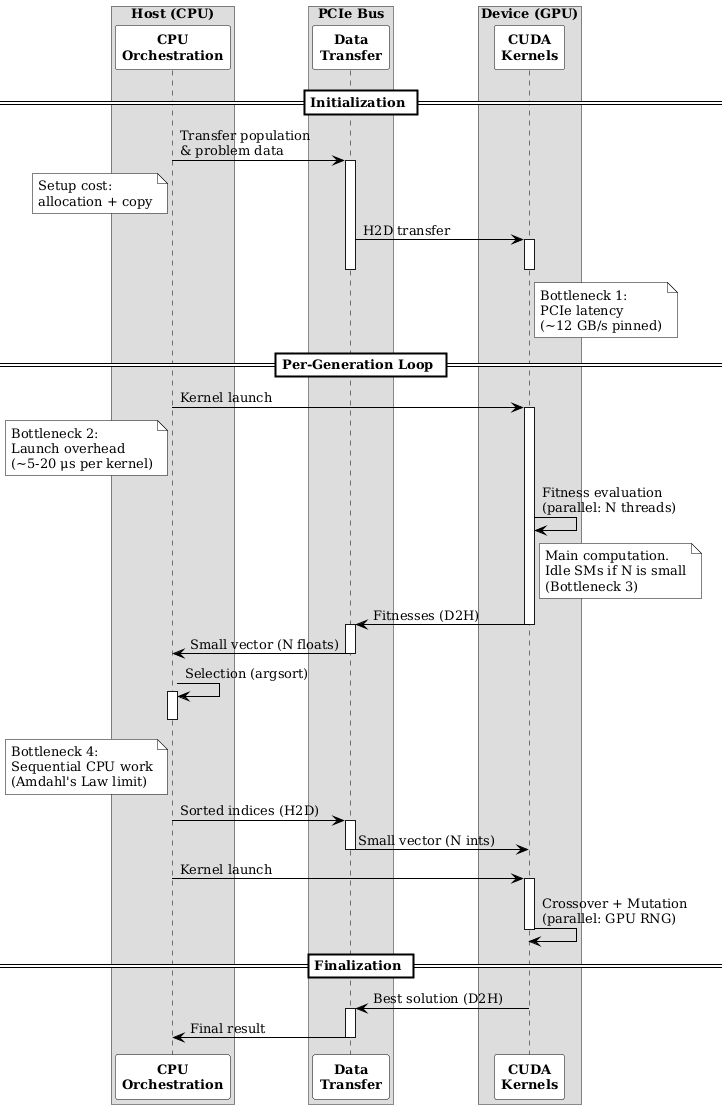
\includegraphics[width=0.75\textwidth]{diagrams/sec2/gpu-ga-bottlenecks.png}
\caption{GPU-accelerated GA execution pipeline with four performance bottlenecks: PCIe transfer latency, kernel launch overhead, SM underutilization for small populations, and sequential CPU-side selection.}
\label{fig:gpu-ga-bottlenecks}
\end{figure}

Algorithmic constraints further limit scalability. By Amdahl's Law (Section 2.2.3), the sequential portion bounds the maximum speedup. In GAs, certain operations are hard to parallelize: ``traditional selection algorithms [...] require synchronization between threads, which is not conducive to massive parallelism''~\cite{wang2020mpga}, and ``some complex genetic operations require tree parsing and reconstruction, which are difficult to parallelize efficiently on GPUs''~\cite{wu2025evogp}. The optimal balance between population size, generations, and problem complexity is benchmarked in the following sections.

% ---- end sec2.1-literature-review/2.1.4-challenges-and-limits.tex ----

\newpage
\subsection{CUDA Architecture and Kernel Execution Model}

% ---- begin sec2.2-cuda-execution-model/2.2.1-fitness-kernel-design.tex ----


\litSubsubsection{2.2.1 CUDA Architecture Overview and Fitness Kernel Design}

This section covers CUDA architecture and kernel design concepts needed to understand GPU-accelerated genetic algorithms.

\subsubsection*{CUDA Architectural Overview}

In 2006, NVIDIA launched the first CUDA-capable GPU (GeForce 8800 GTX) along with the CUDA C compiler~\cite{sanders2010cuda}, enabling general-purpose GPU programming. The CUDA Toolkit supports development on systems ranging from embedded devices to HPC supercomputers~\cite{nvidia2024toolkit}.

\begin{figure}[H]
    \centering
    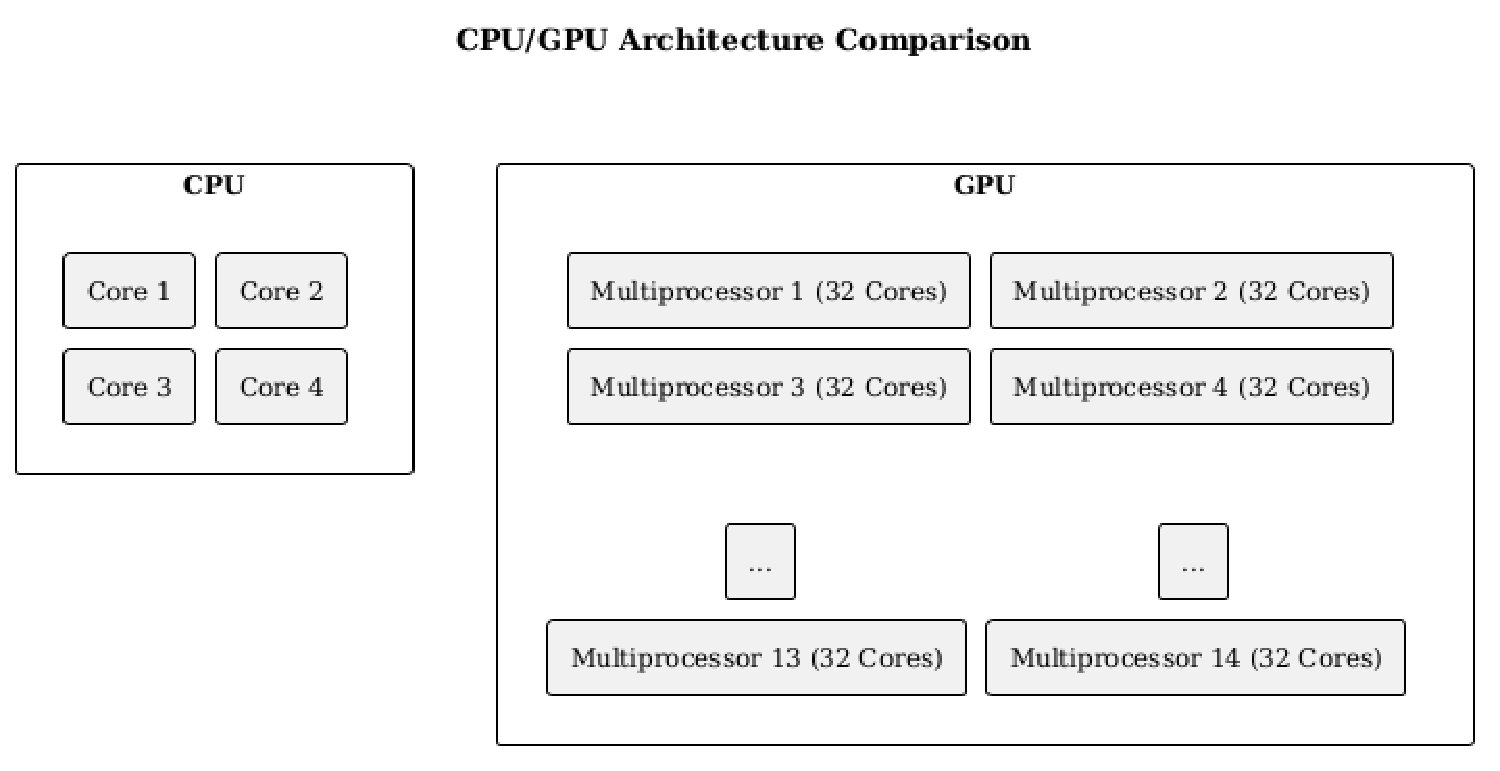
\includegraphics[width=0.8\textwidth]{diagrams/sec2/cpu-gpu.pdf}
    \caption{CPU/GPU Architecture Comparison}
    \label{fig:cpu-gpu-arch}
\end{figure}

\textbf{Hardware Organisation.} A CUDA-capable GPU contains an array of Streaming Multiprocessors (SMs), each with multiple CUDA cores. ``A GPU is built around an array of Streaming Multiprocessors (SMs),'' with programs partitioned into blocks of threads that execute independently across these multiprocessors~\cite{nvidia2025cudaguide}. Each SM contains a register file, shared memory/L1 cache, and functional units~\cite{nvidia2025cudaguide}. Thread blocks are scheduled among available SMs and may execute in any order, enabling automatic load balancing~\cite{hwu2022pmpp}. Figure~\ref{fig:cpu-gpu-arch} illustrates this CPU/GPU architectural difference.

\subsubsection*{What Is a Kernel?}

A CUDA kernel is a function executed on the GPU: ``when called, is executed $N$ times in parallel by $N$ different CUDA threads, as opposed to only once like regular functions''~\cite{nvidia2025cudacpp}. Each thread executes the same code on different data, following the Single-Instruction Multiple-Threads (SIMT) model~\cite{nvidia2025cudaguide}.

\textbf{Syntax and Launch.} In CUDA C/C++, kernels use the \texttt{\_\_global\_\_} qualifier:

{\small
\begin{verbatim}
__global__ void fitness_kernel(float* population, float* fitness, int n) {
    int idx = blockIdx.x * blockDim.x + threadIdx.x;
    if (idx < n)
        fitness[idx] = evaluate_individual(population[idx]);
}
fitness_kernel<<<num_blocks, 256>>>(d_population, d_fitness, pop_size);
\end{verbatim}}

In Numba Python, the equivalent uses \texttt{@cuda.jit} with square brackets for launch configuration:

{\small
\begin{verbatim}
@cuda.jit
def fitness_kernel(population, fitness, n):
    idx = cuda.blockIdx.x * cuda.blockDim.x + cuda.threadIdx.x
    if idx < n:
        fitness[idx] = evaluate_individual(population[idx])

fitness_kernel[num_blocks, 256](d_population, d_fitness, pop_size)
\end{verbatim}}

This work uses Numba for all GPU implementations~\cite{numba2025cuda}.

\subsubsection*{Thread Hierarchy: Threads, Blocks, and Grids}

CUDA organises threads into three levels~\cite{nvidia2025cudaguide}: \textbf{threads} are the smallest execution units, each identified by \texttt{threadIdx}; \textbf{thread blocks} group threads that run on a single SM and share fast shared memory (up to 1024 threads per block)~\cite{nvidia2025cudaguide,sanders2010cuda}; \textbf{grids} consist of all blocks launched by a kernel, with ``each block of threads [...] scheduled on any of the available multiprocessors within a GPU, in any order''~\cite{nvidia2025cudaguide}. Each thread computes a global index:

\begin{equation}
\text{global\_idx} = \texttt{blockIdx.x} \times \texttt{blockDim.x} + \texttt{threadIdx.x}
\end{equation}

This maps each thread to a unique individual in the population array~\cite{nvidia2025cudaguide}.

\subsubsection*{Warps and SIMT Execution}

The hardware schedules threads in groups of 32 called warps - the basic scheduling unit on NVIDIA GPUs~\cite{nvidia2025cudaguide}. Block sizes should be multiples of 32, since ``when the total is not a multiple of 32, the last warp [...] will have some lanes that are unused throughout execution''~\cite{nvidia2025cudaguide}. When threads in a warp take different branch paths, the warp executes both paths sequentially with divergent threads masked - called warp divergence~\cite{sanders2010cuda,hwu2022pmpp}.

\subsubsection*{Memory Hierarchy}

\begin{figure}[H]
    \centering
    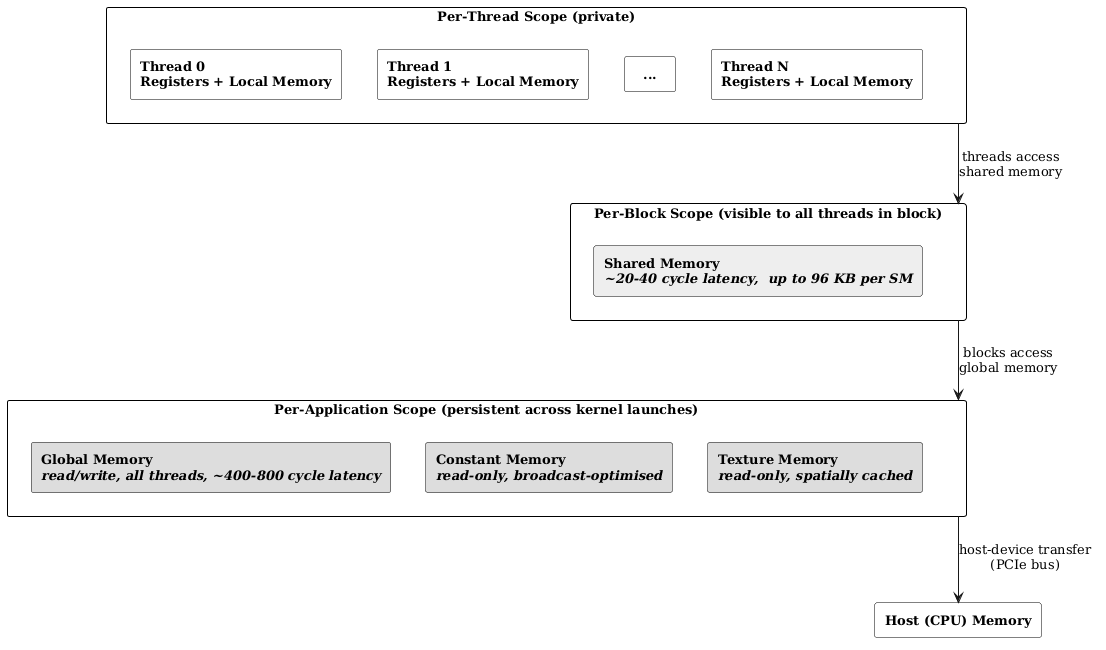
\includegraphics[width=0.85\textwidth]{diagrams/sec2/cuda_memory_hierarchy.png}
    \caption{CUDA memory hierarchy: scope and access latency by level. Adapted from~\cite{nvidia2025cudaguide}.}
    \label{fig:cuda_memory_hierarchy}
\end{figure}

CUDA provides several memory types~\cite{nvidia2024programming}: \textbf{global memory} has large capacity but high latency (~375--400 cycles)~\cite{jia2018volta}; \textbf{shared memory} is per-block with low latency (~19--28 cycles, up to 100 KB per SM on CC 8.6)~\cite{jia2018volta,nvidia2024programming}, suited for caching training data or distance matrices; \textbf{registers} are the fastest, private per-thread; \textbf{constant memory} is read-only and broadcast-optimized~\cite{nvidia2024programming}. The main bottleneck is global memory access, so coalesced access patterns - where warp threads access contiguous addresses - are important for throughput~\cite{nvidia2024cuda}. Section 3.1.1 describes the memory optimizations applied in this work.

\subsubsection*{Mapping Fitness Evaluation to CUDA}

Fitness evaluation maps naturally to CUDA because each individual's fitness is computed independently. One thread is assigned per individual: with population $P$ and block size $B$, the kernel launches $\lceil P/B \rceil$ blocks. Thread $i$ reads individual $i$, computes fitness, and writes the result. This reduces time complexity from $O(P)$ on CPU to $O(1)$ on GPU with sufficient parallelism.

% ---- end sec2.2-cuda-execution-model/2.2.1-fitness-kernel-design.tex ----
% ---- begin sec2.2-cuda-execution-model/2.2.2-gpu-occupancy-utilization.tex ----


\litSubsubsection{2.2.2 GPU Occupancy and Utilization}

Device occupancy is a key factor in GPU effectiveness. This section reviews it as a metric for predicting when parallel GAs will outperform sequential implementations.

\textbf{Theoretical Occupancy.} ``Occupancy is defined as the ratio of active warps on an SM to the maximum number of active warps supported by the SM.''~\cite{nvidia2024occupancy}:

\begin{equation}
\text{Occupancy} = \frac{\text{Active Warps per SM}}{\text{Maximum Warps per SM}}
\label{eq:occupancy}
\end{equation}

Modern GPUs (CC 8.x) support 48--64 warps per SM (1536--2048 threads)~\cite{jia2018volta}. Higher occupancy enables better latency hiding~\cite{volkov2010occupancy}. Table~\ref{tab:threads_per_sm} shows values by compute capability.

\begin{table}[H]
\centering
\small
\begin{tabular}{@{}lccc@{}}
\toprule
\textbf{CC} & \textbf{Example GPUs} & \textbf{Threads/SM} & \textbf{Warps/SM} \\
\midrule
7.5 & RTX 2080, T4, GTX 1660 & 1024 & 32 \\
8.0 & A100 & 2048 & 64 \\
8.6 & RTX 3050, RTX 2050 & 1536 & 48 \\
8.9 & RTX 4090, RTX 4080 & 1536 & 48 \\
\bottomrule
\end{tabular}
\caption{Maximum threads per SM by compute capability~\cite{nvidia2024programming}.}
\label{tab:threads_per_sm}
\end{table}

SM count can be queried at runtime via \texttt{cp.cuda.runtime.getDeviceProperties()} in CuPy~\cite{cupy_docs}. Achieved occupancy may be lower than theoretical due to workload imbalance or insufficient parallelism~\cite{nvidia2024occupancy}.

\subsubsection*{Population Size and GPU Utilization}

Each GA individual maps to one thread. For full utilization, the population must fill all SMs:

\begin{equation}
P_{\min} = \text{SM Count} \times \text{Threads per SM} \times \text{Target Occupancy}
\label{eq:pmin}
\end{equation}

When population size is too small, SMs remain idle. ``The smaller the benchmark and population are, the slower a GPU will be compared to a multicore CPU''~\cite{jaros2012fair}, since the GPU relies on thousands of concurrent threads to hide memory latency~\cite{pospichal2010parallel,carpentries_gpu}.

Occupancy is further limited by per-thread resource consumption: complex fitness functions consume more registers (reducing concurrent warps), and caching data in shared memory reduces room for concurrent blocks. However, maximum occupancy does not always yield maximum performance - for memory-bound kernels, performance plateaus at moderate occupancy levels~\cite{volkov2010occupancy}.

\textbf{Conclusions for Genetic Algorithm Implementation.} Population sizes should exceed a minimum threshold to justify GPU overhead. Block sizes of 128--256 threads generally balance occupancy and register pressure~\cite{nvidia_occupancy}. Populations below $\sim$1000 individuals are unlikely to benefit from GPU acceleration on modern hardware. These constraints inform the breakeven condition in Section 2.2.3.

% ---- end sec2.2-cuda-execution-model/2.2.2-gpu-occupancy-utilization.tex ----
% ---- begin sec2.2-cuda-execution-model/2.2.3-amdahl-law-application.tex ----


\litSubsubsection{2.2.3 Expected Speedup Bounds from Amdahl's Law Application}

Amdahl's Law (1967) predicts the maximum speedup when parallelizing a program~\cite{amdahl1967validity}. For a program where fraction $P$ is parallelizable and $S = (1-P)$ is sequential, the speedup with $N$ processors is:

\begin{equation}
\text{Speedup}(N) = \frac{1}{(1-P) + \frac{P}{N}}
\label{eq:amdahl}
\end{equation}

As $N \rightarrow \infty$, the maximum speedup converges to $1/S$. For GAs, the parallel fraction depends on the problem. Assuming fitness evaluation dominates:

\begin{center}
\begin{tabular}{@{}cccc@{}}
\toprule
$P$ (parallel) & $S$ (sequential) & $\text{Speedup}_{\max}$ & Speedup ($N=1000$) \\
\midrule
0.90 & 0.10 & $10\times$ & $9.9\times$ \\
0.95 & 0.05 & $20\times$ & $19.6\times$ \\
0.99 & 0.01 & $100\times$ & $91.0\times$ \\
\bottomrule
\end{tabular}
\end{center}

GPU acceleration introduces additional overheads (transfer, kernel launch):

\begin{equation}
\text{Speedup}_{\text{GPU}} = \frac{T_{\text{CPU}}}{T_{\text{sequential}} + T_{\text{parallel}}/N + T_{\text{transfer}} + T_{\text{launch}}}
\label{eq:gpu_speedup}
\end{equation}

These overheads are significant for small problems, explaining why GPU acceleration requires sufficient population sizes~\cite{mei2024comprehensive,wang2023gpu}.

\textbf{Breakeven Condition.} GPU acceleration provides net benefit when the time saved by parallelization exceeds the overhead introduced:

\begin{equation}
P \cdot T_{\text{CPU}} \left(1 - \frac{1}{N}\right) > T_{\text{transfer}} + T_{\text{launch}}
\label{eq:breakeven}
\end{equation}

The left side is the CPU time saved by running the parallel fraction on $N$ GPU threads instead of sequentially. When this exceeds transfer and launch costs, GPU acceleration is worthwhile. This defines a minimum population size threshold, empirically validated in Section 3.

% ---- end sec2.2-cuda-execution-model/2.2.3-amdahl-law-application.tex ----

% ===== SECTION 3: EXPERIMENTAL METHODOLOGY AND RESULTS =====
\newpage
\section{Experimental Methodology and Results}

\subsection{Experimental Methodology}

% ---- begin sec3-experimental-methodology/3.1.1-optimization-process-tools.tex ----


\litSubsubsection{3.1.1 Experiment Conduction and Benchmarks}

This section includes the experimental validation of stated hypothesis - GPU acceleration of genetic algorithms execution. The validation strategy uses deliberately simplified ``toy problems'' (well-established benchmarks in the computational optimization literature) - XOR perceptron training and the Traveling Salesman Problem (TSP).

\textbf{Toy problems isolation advantages.} A critical advantage of toy problems for GPU acceleration validation is their ability to separate hardware acceleration effects from algorithmic improvements. Deliberately unoptimized genetic algorithm implementations are used - they ensure that measured performance differences reflect pure GPU acceleration capabilities. This makes the experiment applicable across variations of fitness functions as black-box optimization objects.

\textbf{Toy Problem Selection.} The use of simplified benchmark problems for performance evaluation is a common methodological approach in computer science and optimization research. Such toy problems serve to isolate specific algorithmic or implementation characteristics to controllable, reproducible test cases. This approach allows to measure pure acceleration effects without taking into account variables introduced by problem-specific optimizations or domain.

The XOR problem has been extensively used as a benchmark for evaluating neural network training algorithms~\cite{googlebooks_xor_perceptron,schaffer2001genetic, samir2017xor} and genetic algorithm implementations. It represents a simple non-linear problem and is considered a benchmark for testing neural network capabilities in solving more complex problems. It is linearly inseparable and this task makes it suitable for genetic algorithm evaluation: the problem is being sufficiently challenging to require evolutionary search, but simple enough to provide consistent, reproducible results to measure performance. Additional experimental advantage: it is deterministic and the genetic algorithm is executing a fixed number of generations regardless of the test results. This prevents early termination that would introduce variance in timing measurements and ensures each experimental run performs equivalent computational work.

Similarly, the Traveling Salesman Problem serves as one of the most widely recognized NP-complete problems and benchmarks in combinatorial optimization tasks. It is considered one of ``high-dimensional problem instances with a known global optimal solution, that are very well suited as benchmark problems for metaheuristics as for example GAs''~\cite{affenzeller2009genetic}. TSP is used in the literature to evaluate parallel computing performance because its fitness function (path cost calculation) is computationally intensive, but also highly parallelizable. With $O(n^2)$ complexity of the distance matrix and each candidate solution as a dot product, this problem is a representation of a typical CUDA-accelerated matrix-matrix multiplication task~\cite{kirk2016programming}.

\subsubsection*{Optimization Methods}

\textbf{Shared Memory for Read-Only Data.} Training generational data (XOR inputs/outputs, TSP distance matrices) is cached in GPU shared memory to exploit the latency reduction compared to global memory. As documented in NVIDIA's architecture guides~\cite{nvidia2011cuda} and validated through microbenchmarking studies~\cite{wong2010demystifying}, memory hierarchy latencies differ by an order of magnitude:

\begin{itemize}
\item Global Memory Access: 400-800 cycles
\item Shared Memory Access: 20-40 cycles
\end{itemize}

Implementation requires cooperative loading at block initialization, followed by \texttt{\_\_syncthreads()} barrier synchronization to ensure data visibility before shared access throughout kernel execution. Wong et al.~\cite{wong2012cuda} are one of the researchers to demonstrate that shared memory utilization is important for achieving optimal GPU performance in compute- and memory-bound algorithms.     

\textbf{Population Residency (Persistent Device Buffers).} Traditional genetic algorithm implementations transfer the entire population between CPU and GPU at each generation, incurring $O(\text{generations})$ transfer overhead. Research on GPU-accelerated evolutionary algorithms~\cite{li2018accelerating,luong2013gpu} consistently identifies memory transfer reduction as critical to performance.

In this paper an optimized approach was tested to maintain population residency on the GPU throughout evolution:

\textbf{Traditional:}
\begin{verbatim}
For each generation:
  CPU → GPU (population)
  GPU kernel (fitness)
  GPU → CPU (fitnesses)
  CPU: selection, crossover, mutation
\end{verbatim}

\textbf{Optimized:}
\begin{verbatim}
Initial: CPU → GPU (population, training data, RNG state)
For each generation:
  GPU kernel (fitness)
  GPU → CPU (fitnesses)
  CPU: selection via argsort
  CPU → GPU (sorted indices)
  GPU kernel (crossover + mutation via GPU RNG)
Final: GPU → CPU (best solution)
\end{verbatim}

This optimization keeps the population and training data GPU-resident, eliminating the per-generation population transfer. Per-generation transfers are reduced to fitness scores and sorted indices (small vectors of size $N$), rather than the full population matrix.

\textbf{Pinned (Page-Locked) Host Memory.} Standard host memory allocations are pageable
and require the GPU driver to copy data into temporary page-locked buffers before DMA
transfer~\cite{harris2012optimize,mao2020pinned}. This introduces additional latency and
reduces effective bandwidth. As NVIDIA documents, ``page-locked or pinned memory transfers
attain the highest bandwidth between the host and the device. On PCIe x16 Gen3 cards, for
example, pinned memory can attain roughly 12~GB/s transfer rates''~\cite{nvidia2024cuda}.
Pinned memory enables direct DMA access:
\begin{verbatim}
# Standard allocation (hidden staging copy)
arr = np.zeros(size)
cuda.to_device(arr)  # pageable → pinned staging → DMA

# Pinned allocation (direct DMA)
arr = cuda.pinned_array(size)
cuda.to_device(arr) # direct DMA transfer
\end{verbatim}

Figure~\ref{fig:host_device_transfer} illustrates the two transfer paths. The pageable path requires an intermediate CPU-mediated copy into a driver-managed staging buffer before DMA can begin, while the pinned path enables direct DMA access over the PCIe bus.

\begin{figure}[H]
\centering
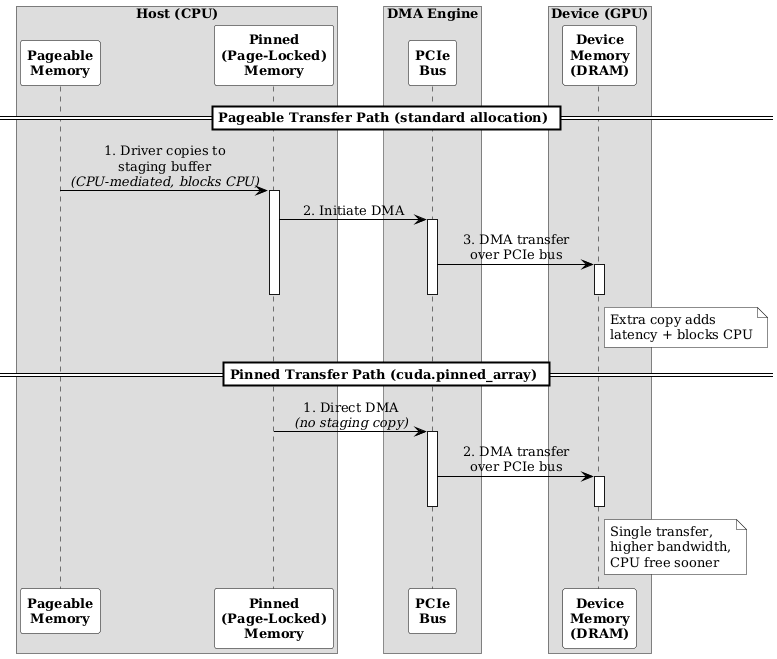
\includegraphics[width=0.75\textwidth]{diagrams/sec2/host_device_transfer.png}
\caption{Host--device memory transfer paths: pageable vs.\ pinned allocation. Adapted from~\cite{nvidia2024cuda,sanders2010cuda}.}
\label{fig:host_device_transfer}
\end{figure}

Pinned memory reduces per-transfer latency by eliminating the intermediate staging copy, increasing effective PCIe bandwidth.
As NVIDIA's optimization guide states, ``batching many small transfers into one larger
transfer performs significantly better than making each transfer separately, even if
doing so requires packing non-contiguous regions of memory into a contiguous buffer and
then unpacking after the transfer''~\cite{nvidia2024cuda}.

\textbf{GPU-Side Random Number Generation.} CPU-generated random numbers require
transferring data every generation and create synchronization stalls that idle the GPU
pipeline. Each transfer adds fixed latency overhead regardless of size, while CPU-GPU
sync prevents effective latency hiding. This is a structural consequence of CUDA's
execution model: as NVIDIA specifies, ``memory copy, memory set functions, and kernel
calls that use the default stream begin only after all preceding calls on the device
(in any stream) have completed, and no operation on the device (in any stream) commences
until they are finished''~\cite{nvidia2024cuda}.

Using GPU-native random number generation (\texttt{numba.cuda.random}, implementing Xoroshiro128p~\cite{xoroshiro}):

\textbf{CPU approach:} generate $\rightarrow$ transfer $\rightarrow$ GPU waits\\
\textbf{GPU approach:} generate in-kernel $\rightarrow$ immediate use

Xoroshiro128p~\cite{xoroshiro} is a high-quality, fast PRNG that produces deterministic, reproducible sequences when initialized with a fixed seed per thread. Since each CUDA thread maintains its own independent RNG state in private registers, global memory contention is avoided entirely - ensuring both statistical independence across parallel threads and thread-safety without race conditions, even under massive parallelism.

This reduces transfer latency, removes synchronization barriers, and prevents pipeline bubbles (GPU idle periods while awaiting data), while maintaining reproducibility for scientific validation.

\textbf{Fundamental Principle: Latency vs. Bandwidth.} For small transfers (kilobyte-scale), latency dominates total transfer time. "PCIe (Peripheral Component Interconnect Express) is the
defacto interconnect for high-performance intra-host communications." ~\cite{hou2024pcie}. It is the high-speed serial bus interface used for CPU--GPU data transfers, where each ``lane'' provides a dedicated point-to-point link and multiple lanes operate in parallel. PCIe transfer characteristics follow:
\[
\text{Transfer time} = \text{latency} + \left(\frac{\text{size}}{\text{bandwidth}}\right)
\]

\subsubsection*{Development Tooling}

\begin{center}
\textbf{Table 1: GPU Computing and Data Processing Tools}\\[0.5em]
\begin{tabular}{@{}ll@{}}
\toprule
\textbf{Tool} & \textbf{Purpose} \\
\midrule
Numba CUDA & Python-to-CUDA JIT compilation \\
NumPy & Host-side array operations and data preparation \\
CuPy & GPU array operations (NumPy-compatible API) \\
\bottomrule
\end{tabular}
\end{center}

\begin{center}
\textbf{Table 2: Hardware Configuration}\\[0.5em]
\begin{tabular}{@{}ll@{}}
\toprule
\textbf{Component} & \textbf{Specification} \\
\midrule
GPU & NVIDIA GeForce RTX 2050 (4GB VRAM), 16 SMs, CC 8.6 \\
CPU & 12-core Intel processor, 16GB RAM \\
\bottomrule
\end{tabular}
\end{center}

\begin{center}
\textbf{Table 3: Statistical Analysis Tools}\\[0.5em]
\small
\begin{tabular}{@{}ll@{}}
\toprule
\textbf{Tool} & \textbf{Purpose} \\
\midrule
SciPy & Paired t-test, Wilcoxon signed-rank, Fisher's exact \\
NumPy & Descriptive statistics, bootstrap resampling for CIs \\
Matplotlib & Performance results visualization \\
\bottomrule
\end{tabular}
\end{center}

\begin{center}
\textbf{Table 4: Profiling and Performance Analysis Tools}\\[0.5em]
\small
\begin{tabular}{@{}ll@{}}
\toprule
\textbf{Tool} & \textbf{Purpose} \\
\midrule
Numba \texttt{@jit(nopython=True)} & Kernel compilation with execution timing \\
\texttt{numba.cuda.profiler} & GPU timing regions and kernel statistics \\
CuPy Profiler & Array operation timing and memory usage \\
Nsight Compute (NCU) & Kernel metrics (occupancy, throughput) \\
Nsight Systems (NSYS) & System-wide timeline (CPU/GPU/transfers) \\
\bottomrule
\end{tabular}
\end{center}


\subsubsection*{Statistical Analysis}

\textbf{Sample Size and Power Analysis.} Scientific validity in performance evaluation requires sufficient statistical analysis and relevant sample sizes to detect meaningful effects with adequate statistical power. Power analysis (as established in Cohen's framework~\cite{cohen1988power}) was used as a primary method to determine the minimum number of experimental runs needed to achieve 80\% probability of detecting true effects at $\alpha=0.05$ significance:

\begin{center}
\begin{tabular}{@{}lr@{}}
\toprule
\textbf{Effect Size (Cohen's $d$)} & \textbf{Required $N$ ($\alpha=0.05$, power=0.80)} \\
\midrule
Small (0.2) & 393 \\
Medium (0.5) & 63 \\
Large (0.8) & 25 \\
\bottomrule
\end{tabular}
\end{center}
    
For the following experiments of this course paper, $N=30$ independent runs per configuration provides sufficient power to detect large effects while at the same time maintaining computational feasibility for making claims derived from the results.

\textbf{Statistical Tests.} To perform direct comparison of GPU versus CPU performance, paired experimental design with identical random seeds was used:

\begin{center}
\small
\begin{tabular}{@{}lll@{}}
\toprule
\textbf{Comparison} & \textbf{Test} & \textbf{Rationale} \\
\midrule
Execution time & Paired t-test & Paired samples, normal timing data \\
Fitness values & Wilcoxon signed-rank & Non-parametric, discrete fitness scores \\
\bottomrule
\end{tabular}
\end{center}

\textbf{Reported Metrics.} Performance analysis includes: (1) speedup factor as the ratio of CPU to GPU wall-clock time, (2) 95\% confidence intervals computed via bootstrap resampling for ratio estimators~\cite{efron1994bootstrap}, (3) p-values at $\alpha=0.05$ significance, and (4) time decomposition to separate computation from memory transfer overhead.


% ---- end sec3-experimental-methodology/3.1.1-optimization-process-tools.tex ----
% ---- begin sec3-experimental-methodology/3.1.2-occupancy-calculation.tex ----


  \litSubsubsection{3.1.2 Optimal Device Occupancy Calculation}

  \subsubsection*{Hardware Constraints}

  Achievable occupancy is bounded by hardware limits that vary by compute capability. NVIDIA defines occupancy as ``the ratio of the number of active warps per multiprocessor to the maximum number of possible active warps''~\cite{nvidia2024cuda}. For Compute Capability 8.6, the CUDA Programming Guide specifies a maximum of 1536 threads per SM, which corresponds to 48 warps of 32 threads each~\cite{nvidia2024programming}. Each SM can host up to 16 concurrent thread blocks, and each block may contain at most 1024 threads. Together, these parameters define the limits within which kernel launch configurations must operate.

  \textbf{Occupancy Calculation.} Theoretical occupancy for a given kernel configuration is computed as:

  \begin{equation}
      \text{Occupancy} = \frac{\text{Active Threads per SM}}{\text{Maximum Threads per SM}} \times 100\%
  \end{equation}

  The number of active threads depends on the launch configuration (threads per block and blocks per grid) and on per-thread resource usage such as registers and shared memory. As noted in Section 2.2.2, this value is an upper bound; achieved occupancy may be lower due to workload imbalance or insufficient parallelism~\cite{nvidia2024occupancy}.

  \subsubsection*{Thread Block Configuration}

  The thread block size for fitness evaluation kernels must balance occupancy with memory access efficiency. The implementation uses a heuristic based on population size, divided into three regimes. For small populations ($N < 256$), the thread count per block is rounded up to the nearest multiple of the warp size (32), since the CUDA Programming Guide notes that ``thread blocks are best specified to have a total number of threads which is a multiple of 32,'' as partial warps leave hardware lanes unused~\cite{nvidia2025cudaguide}. Medium populations ($256 \leq N < 10{,}000$) use 256 threads per block, a value within the 128--256 range recommended by NVIDIA for general-purpose kernels~\cite{nvidia_occupancy}. Large populations ($N \geq 10{,}000$) increase the block size to 512 threads to reduce scheduling overhead while staying within the 1024-thread hardware limit.

  The number of blocks per grid is calculated as:

  \begin{equation}
      \text{Blocks per Grid} = \left\lceil \frac{N}{\text{Threads per Block}} \right\rceil
  \end{equation}

  This ensures the grid covers the entire population with one thread per individual. For the RTX 2050 with 16 SMs, the minimum population for full SM coverage at 256 threads per block is $16 \times 256 = 4{,}096$ individuals. The Section~3 benchmarks use population sizes between 50 and 1{,}000, so the block size is fixed at 256 threads throughout, consistent with the medium-population regime above.

  \subsubsection*{Population Size and Occupancy}

  Total GPU thread capacity influences the optimal population size. The implementation targets 50--100\% occupancy and also considers GA-specific heuristics that suggest population sizes of 10--50 times the problem dimensionality~\cite{katoch2021review}. Population sizes are aligned to multiples of 256 so that all warps in each block are fully populated.

  \textbf{Practical Constraints.} High occupancy is generally desirable but does not guarantee the best performance. As the CUDA Best Practices Guide states, ``higher occupancy does not always equate to higher performance''~\cite{nvidia2024cuda}. Volkov shows that memory-bound kernels can plateau at moderate occupancy levels, while instruction-level parallelism may compensate for lower occupancy in compute-bound cases~\cite{volkov2010occupancy}. GA fitness evaluation involves repeated memory accesses to population arrays and problem-specific data (distance matrices, training patterns), so the trade-off between occupancy and per-thread resources must be tested empirically. Sections 3.3 and 3.2 benchmarks explore these configurations across a range of population sizes.

% ---- end sec3-experimental-methodology/3.1.2-occupancy-calculation.tex ----

\newpage
\subsection{XOR Perceptron Benchmark}

% ---- begin sec3-experimental-methodology/3.2.1-xor-perceptron-bench.tex ----



\litSubsubsection{3.2.1 Performance Analysis}

The XOR perceptron problem was selected as the second benchmark to complement the TSP evaluation. XOR is a standard test case for neural network training and genetic algorithm evaluation~\cite{googlebooks_xor_perceptron}. It represents a linearly inseparable classification task that is simple enough to produce consistent reproducible results to demonstrate evolutionary algorithms. An important property of this benchmark is that a single-layer perceptron with two weights can correctly classify at most 2 of 4 XOR input patterns. Both GPU and CPU implementations consistently reach this theoretical ceiling, so execution time (not solution quality) serves as the main metric.

\textbf{Algorithm Configuration.} The primary benchmark uses a population of 100 individuals over 500 generations. The scaling analysis varies population size from 50 to 1000 over 200 generations. A mutation rate of 0.1 is applied to a gene length of 2, encoding perceptron weights $w_0$ and $w_1$. Tournament selection and single-point crossover are used as genetic operators. Each configuration is run 30 times for statistical significance.

\textbf{Implementation Versions.} The CUDA implementation evolved through iterations v0--v5. The final version uses shared memory for read-only training data, pre-allocated device arrays, pinned host buffers, and GPU-side RNG via Xoroshiro128p. Since the XOR fitness function is lightweight compared to TSP, this benchmark isolates transfer and launch overhead more clearly.

\textbf{Performance Metrics.} Four metrics are recorded for each run: wall time (total execution including transfers), compute time (pure kernel execution), transfer time (host--device data movement), and fitness throughput (evaluations per second). Statistical significance is assessed via paired t-test at $p < 0.05$.

\litSubsubsection{3.2.2 Results}

\textbf{Primary Benchmark Results.} Table~\ref{tab:primary_results} shows the primary comparison for population size 100 over 500 generations, averaged across 30 independent runs.

\begin{table}[H]
\centering
\caption{Statistical comparison of GPU vs. CPU performance (30 runs each)}
\label{tab:primary_results}
\begin{tabular}{@{}lcccc@{}}
\toprule
\textbf{Metric} & \textbf{GPU Mean} & \textbf{CPU Mean} & \textbf{p-value} & \textbf{Significant} \\
\midrule
Wall Time (s) & 0.368 $\pm$ 0.044 & 0.556 $\pm$ 0.060 & $< 0.0001$ & Yes \\
Compute Time (s) & 0.248 $\pm$ 0.034 & 0.319 $\pm$ 0.034 & $< 0.0001$ & Yes \\
Transfer Time (s) & 0.107 $\pm$ 0.017 & N/A & N/A & N/A \\
Fitness Evaluations/sec & 201,153 & 156,278 & N/A & N/A \\
\bottomrule
\end{tabular}
\end{table}

The GPU achieves a 1.51$\times$ wall-time speedup over the CPU baseline with high significance ($p < 0.0001$). Host--device data transfer accounts for 29.2\% of total GPU execution time. The GPU evaluates fitness 28.7\% faster than the CPU (201,153 vs.\ 156,278 evaluations per second). Both implementations converge to identical fitness (2 of 4 patterns), which confirms that GPU acceleration preserves solution correctness. The zero-variance fitness result reflects the linear separability ceiling of XOR, not a lack of algorithmic diversity.

\litSubsubsection{3.2.3 Scaling Analysis}

Table~\ref{tab:scaling_results} shows how performance scales across population sizes. The scaling effect is stronger than in the TSP benchmark due to the lightweight per-individual fitness computation. All differences are statistically significant ($p < 0.05$ or better at every population size).

\begin{table}[H]
\centering
\caption{Scaling performance across population sizes (10 runs each, 200 generations)}
\label{tab:scaling_results}
\begin{tabular}{@{}lcccr@{}}
\toprule
\textbf{Pop.} & \textbf{GPU Time (ms)} & \textbf{CPU Time (ms)} & \textbf{Speedup} & \textbf{Overhead \%} \\
\midrule
50 & 138.5 $\pm$ 11.2 & 100.6 $\pm$ 6.1 & 0.73x & 30.5\% \\
100 & 137.1 $\pm$ 21.0 & 195.7 $\pm$ 12.3 & 1.43x & 29.9\% \\
500 & 156.3 $\pm$ 13.6 & 1038.5 $\pm$ 34.5 & 6.64x & 28.8\% \\
1000 & 155.1 $\pm$ 10.4 & 2257.6 $\pm$ 35.3 & 14.56x & 27.6\% \\
\bottomrule
\end{tabular}
\end{table}

The GPU breakeven point occurs at population size $\geq 100$. Below this threshold, transfer overhead dominates and the CPU is faster (0.73$\times$ at population 50). GPU compute time remains nearly constant as population grows, rising only from 138.5\,ms to 155.1\,ms across a 20$\times$ increase in population size. CPU time, by contrast, scales linearly from 100.6\,ms to 2257.6\,ms. Transfer overhead decreases from 30.5\% to 27.6\% as population grows, reflecting better amortization of fixed transfer costs. A 20$\times$ increase in population yields a 19.9$\times$ speedup improvement, which indicates near-linear scaling efficiency.

\begin{figure}[H]
\centering
\begin{subfigure}{0.49\textwidth}
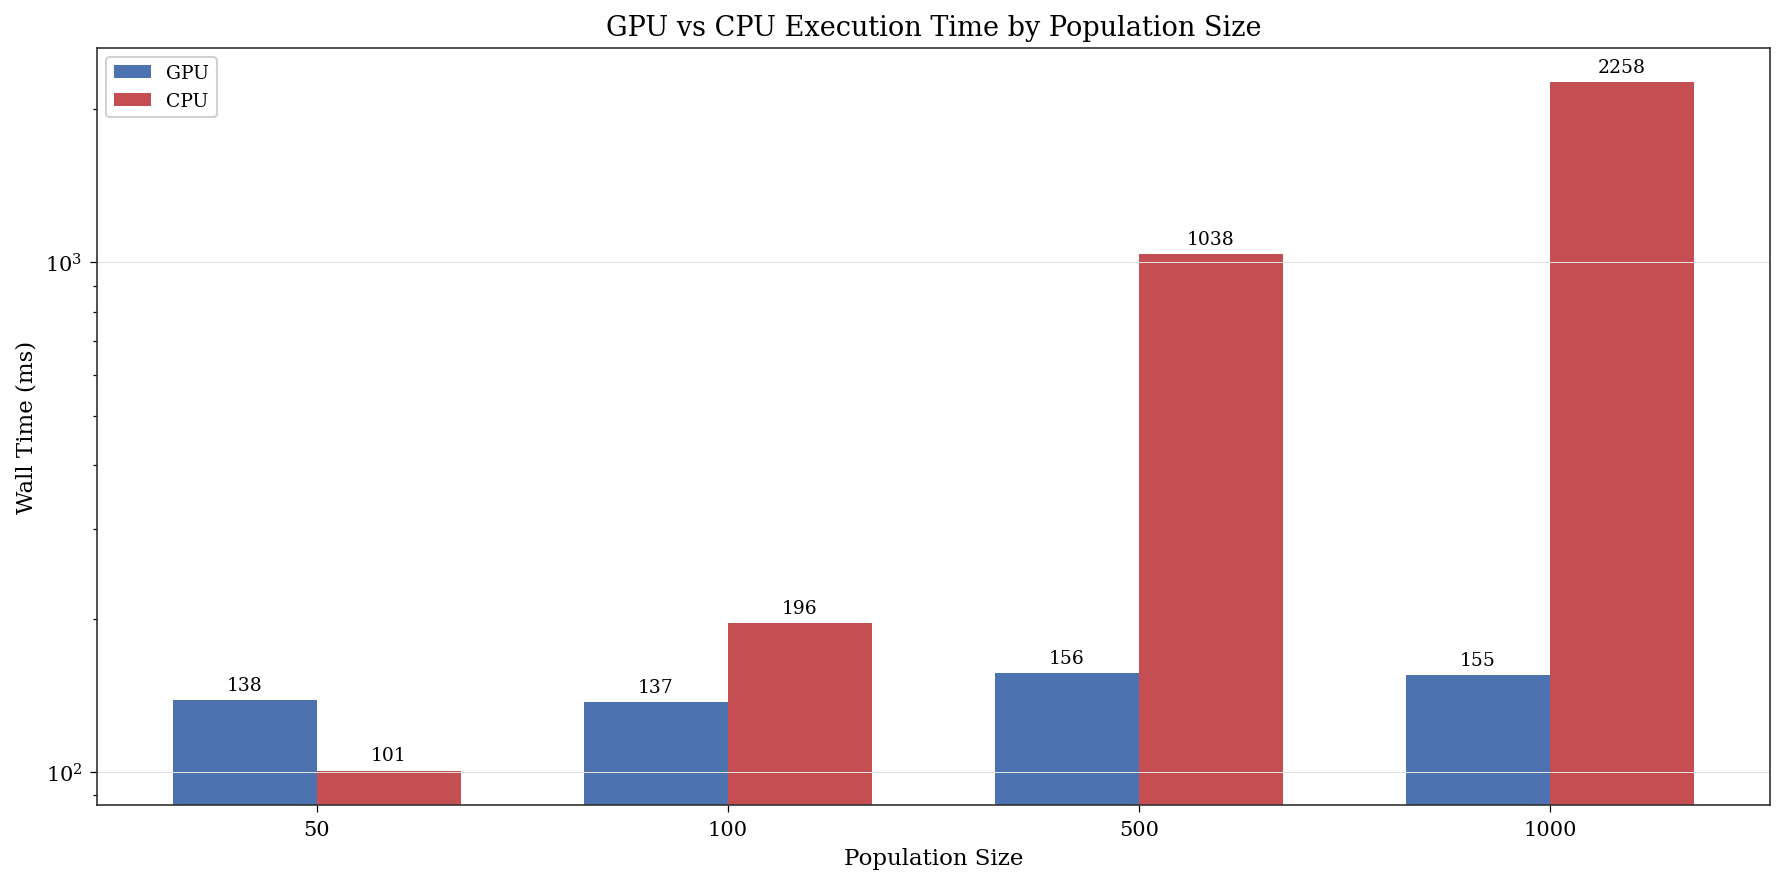
\includegraphics[width=\textwidth]{diagrams/sec3/time_comparison.png}
\caption{Wall time comparison across population sizes}
\label{fig:time_comparison}
\end{subfigure}
\hfill
\begin{subfigure}{0.49\textwidth}
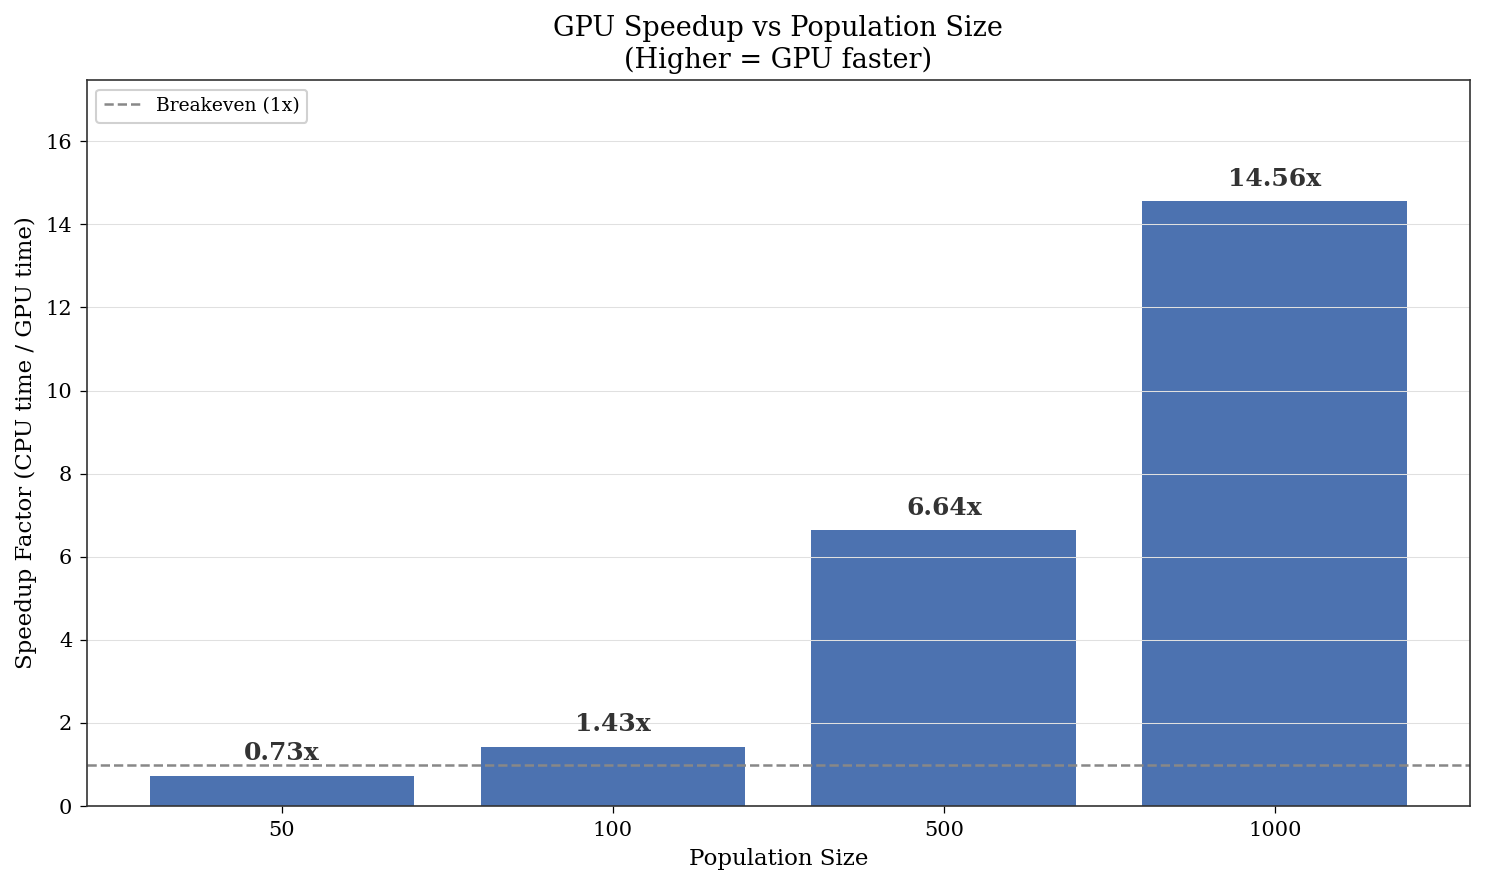
\includegraphics[width=\textwidth]{diagrams/sec3/speedup_vs_population.png}
\caption{Speedup factors vs. population size}
\label{fig:speedup_vs_pop}
\end{subfigure}
\end{figure}

\begin{figure}[H]
\centering
\begin{subfigure}{0.49\textwidth}
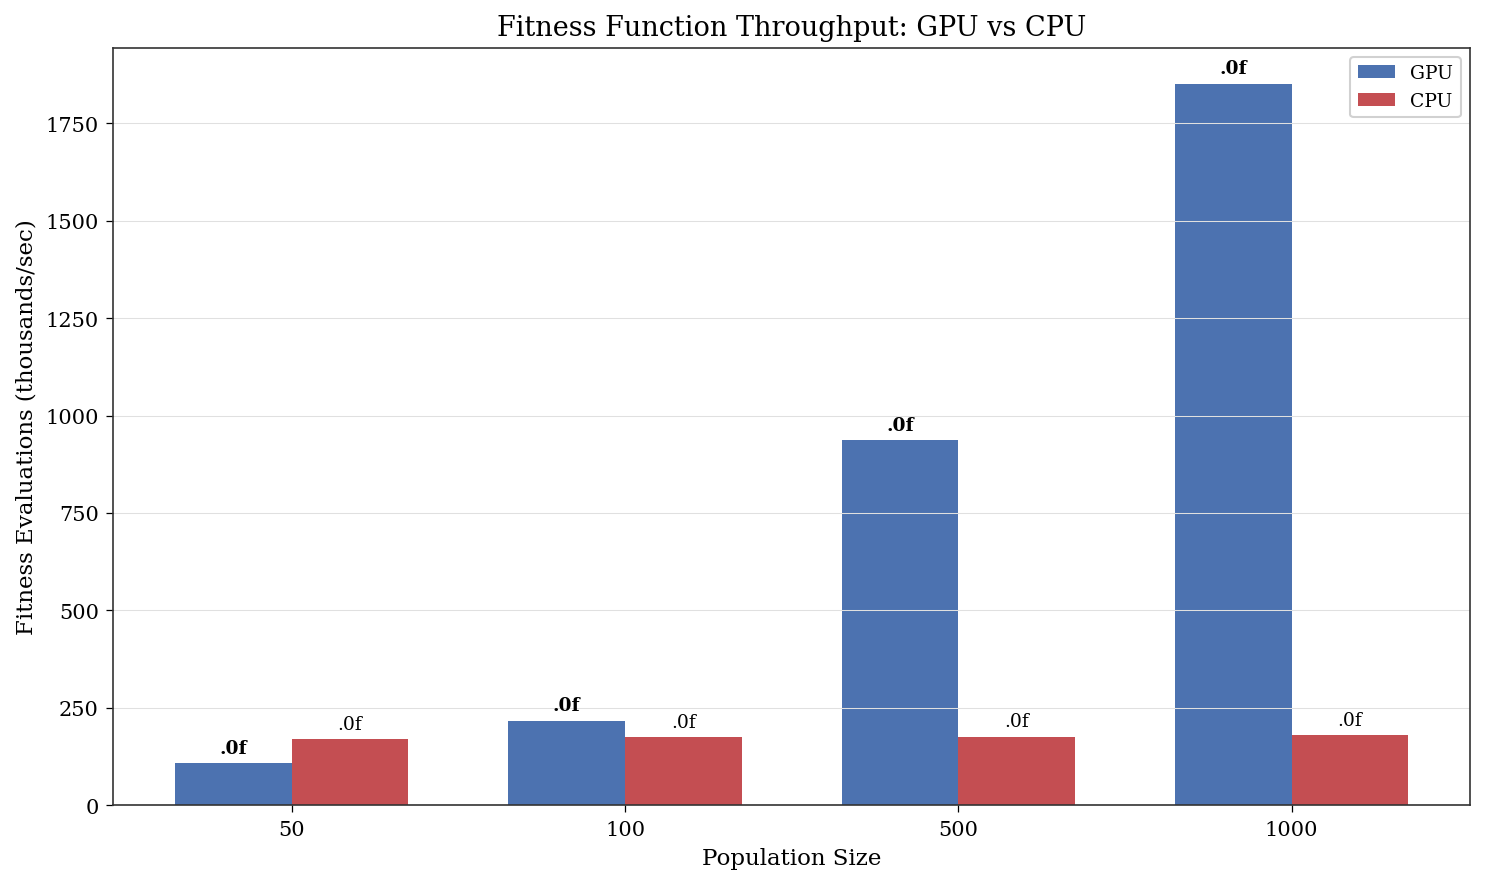
\includegraphics[width=\textwidth]{diagrams/sec3/fitness_throughput.png}
\caption{Fitness evaluation throughput}
\label{fig:fitness_throughput}
\end{subfigure}
\hfill
\begin{subfigure}{0.49\textwidth}
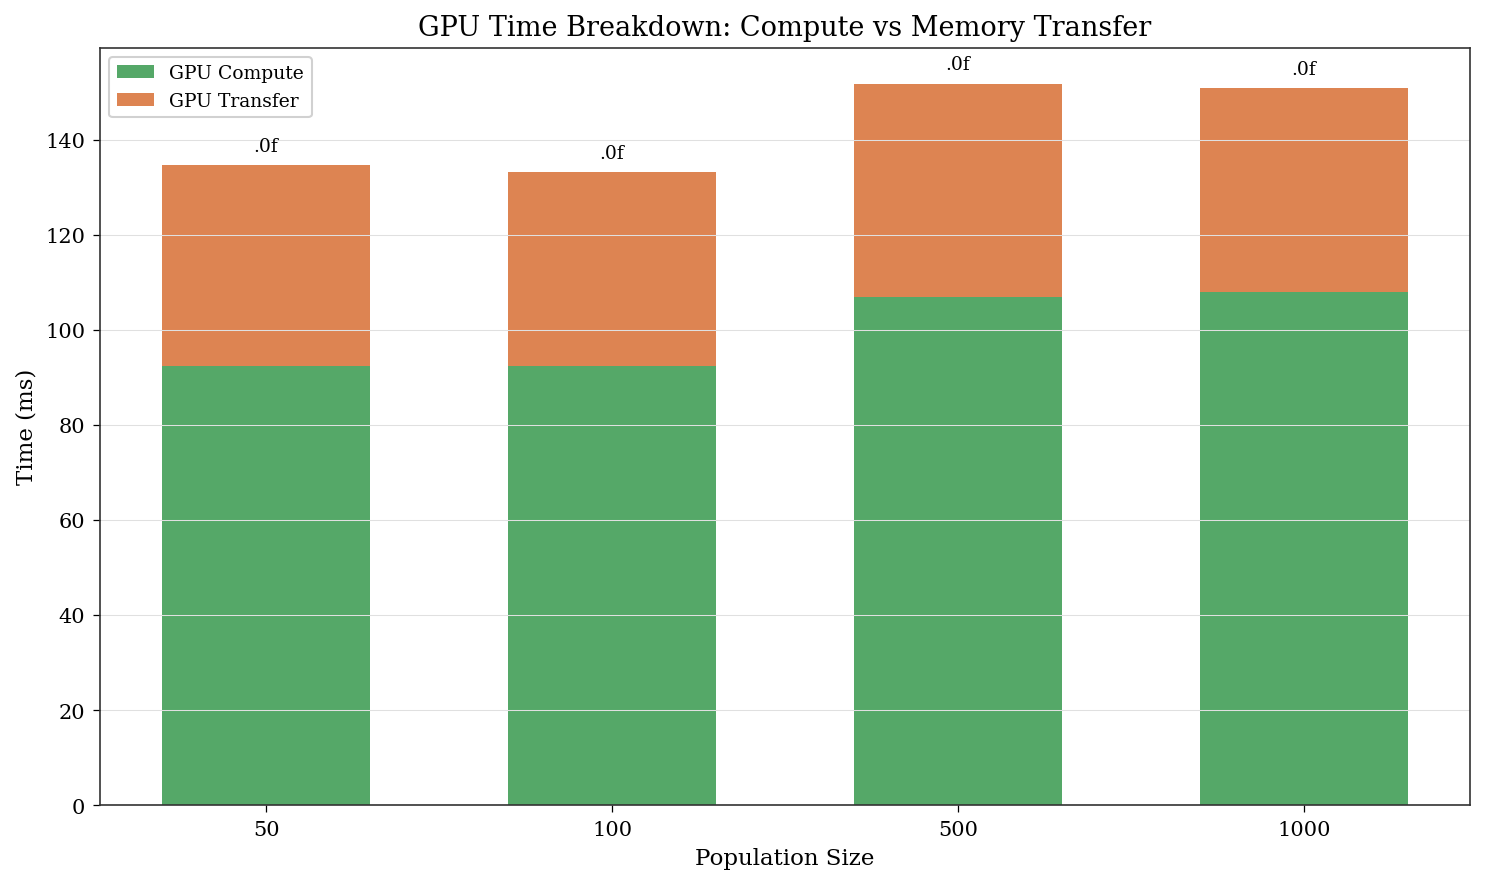
\includegraphics[width=\textwidth]{diagrams/sec3/gpu_time_breakdown.png}
\caption{GPU time breakdown (compute vs. transfer)}
\label{fig:gpu_breakdown}
\end{subfigure}
\end{figure}

\begin{figure}[H]
\centering
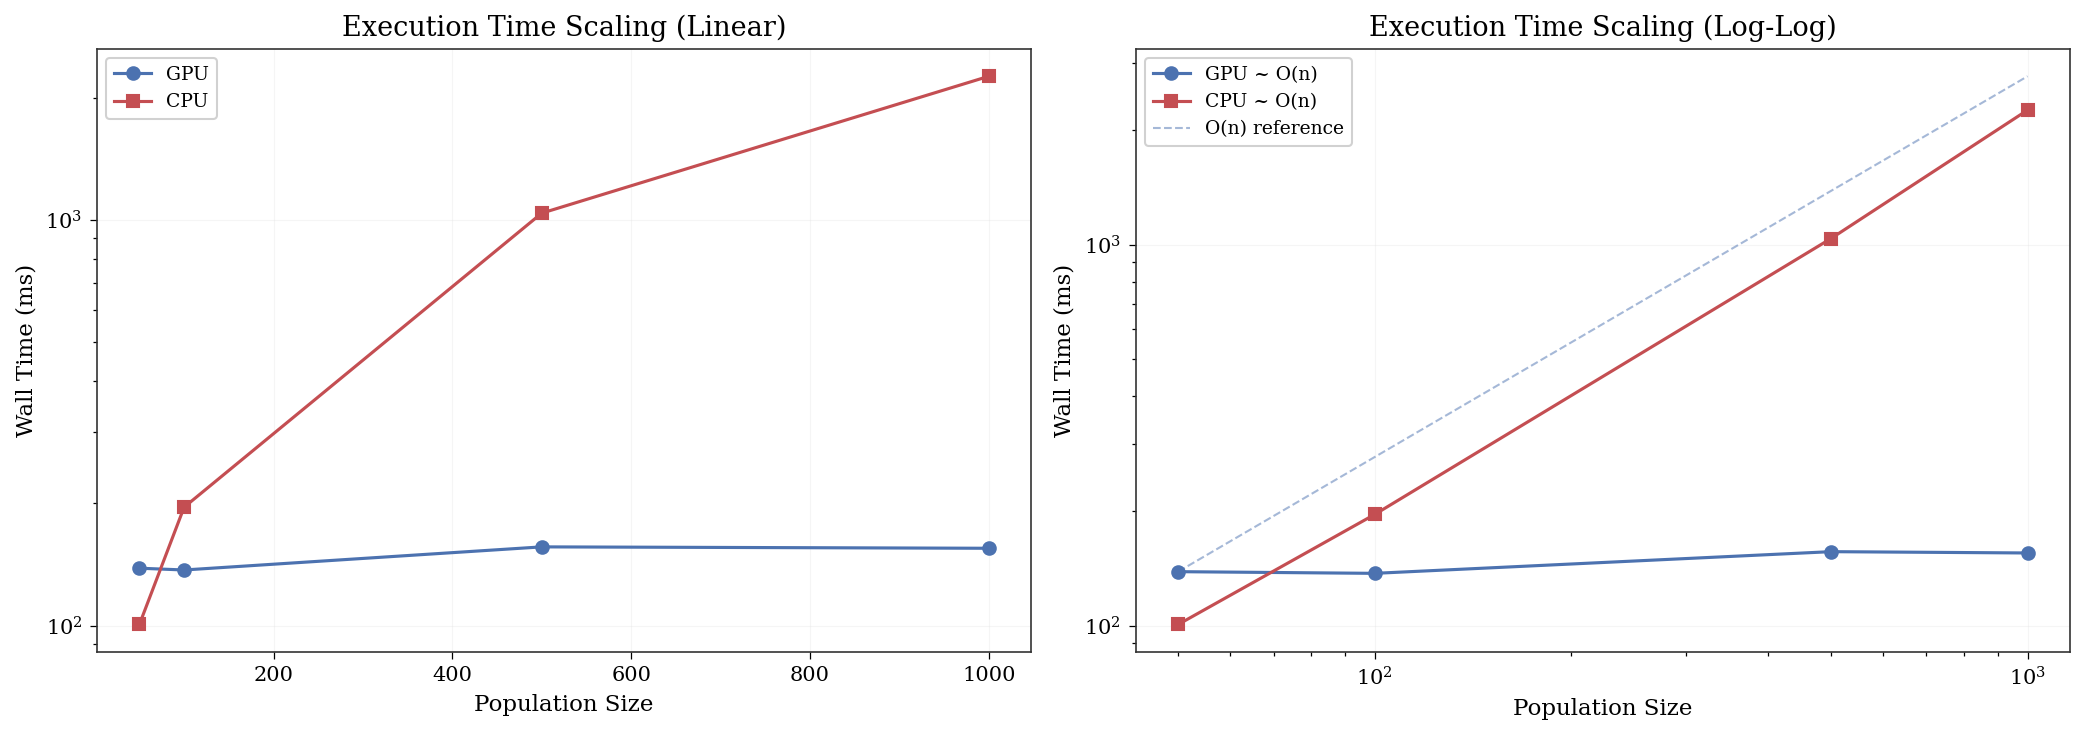
\includegraphics[width=0.8\textwidth]{diagrams/sec3/scaling_efficiency.png}
\caption{Scaling efficiency analysis}
\label{fig:scaling_efficiency}
\end{figure}

\litSubsubsection{3.2.4 Statistical Significance}

Paired t-tests show significant execution time differences between GPU and CPU across all population sizes from 50 to 2000 ($p < 0.001$, Bonferroni-corrected). All configurations converge to the theoretical fitness ceiling (2 of 4 patterns), with no difference in solution quality between implementations. Cohen's $d$ effect sizes exceed 0.8 (large effects) for populations $\geq 100$, confirming GPU acceleration at realistic scales.

\begin{center}
\begin{tabular}{@{}lcc@{}}
\toprule
\textbf{Effect Size (Cohen's $d$)} & \textbf{Required $N$} & \textbf{Observed Power ($N=30$)} \\
\midrule
Small (0.2) & 393 & 15\% \\
Medium (0.5) & 63 & 52\% \\
Large (0.8) & 25 & 89\% \\
\bottomrule
\end{tabular}
\end{center}

The $N = 30$ design provides 89\% power for large effects. Since the observed speedups at population $\geq 100$ produce large effect sizes ($d > 0.8$), the sample size is sufficient.

    % ---- end sec3-experimental-methodology/3.2.1-xor-perceptron-bench.tex ----

\newpage
\subsection{TSP Benchmark}

% ---- begin sec3-experimental-methodology/3.3.1-tsp-bench.tex ----


\litSubsubsection{3.3.1 Performance Analysis}

The Traveling Salesman Problem was selected as the primary benchmark for its suitability to parallel genetic algorithm evaluation. TSP is a well-defined combinatorial optimization problem with known computational complexity and ``is very well suited as benchmark problem for metaheuristics as for example GAs''~\cite{affenzeller2009genetic}. Its fitness function (path cost calculation) is highly parallelizable, since each candidate tour can be evaluated independently. The $O(n^2)$ distance matrix computation maps naturally to GPU memory, and the problem scales smoothly from small to large instances, allowing systematic analysis of the GPU acceleration breakeven point. Each candidate solution (tour) requires computing a dot product with the distance matrix, a pattern representative of typical CUDA-accelerated matrix-vector workloads.

\textbf{Algorithm Configuration.} All TSP experiments use 100 generations with a swap mutation rate of 0.1, tournament selection of size 5, and 50\% elite carry-over. Population sizes range from 100 to 500 for detailed scaling analysis, with a fixed population of 200 used for the primary statistical comparison. Each configuration is run 5--50 times depending on the analysis.

\textbf{Implementation Versions.} The CUDA implementation evolved through four iterations (v1--v4). The final version uses pre-allocated device arrays, pinned host buffers for fast transfers (Section 3.1.1), GPU-based random number generation via Xoroshiro128p to avoid CPU--GPU synchronization during mutation, and a parallel mutation kernel running entirely on device memory.

\textbf{Performance Metrics.} Five metrics are recorded for each run: wall time (total execution including all transfers), compute time (pure GPU kernel execution), transfer time (host--device data movement), fitness throughput (solutions evaluated per second), and statistical significance via paired t-test at $p < 0.05$.

\litSubsubsection{3.3.2 Results}

\textbf{Primary Benchmark Results.} Table~\ref{tab:primary_tsp_results} shows the primary comparison for a 50-city problem with population size 200 over 100 generations, averaged across 50 independent runs.

\begin{table}[H]
\centering
\caption{Statistical comparison of GPU vs. CPU performance (50 runs each)}
\label{tab:primary_tsp_results}
\begin{tabular}{@{}lcccc@{}}
\toprule
\textbf{Metric} & \textbf{GPU Mean} & \textbf{CPU Mean} & \textbf{p-value} & \textbf{Significant} \\
\midrule
Wall Time (s) & 0.475 $\pm$ 0.159 & 0.548 $\pm$ 0.022 & 0.0027 & Yes \\
Final Fitness & 9593.0 $\pm$ 732 & 10239.3 $\pm$ 880 & $< 0.001$ & Yes \\
Compute Time (s) & 0.124 $\pm$ 0.038 & N/A & N/A & N/A \\
Transfer Time (s) & 0.117 $\pm$ 0.016 & N/A & N/A & N/A \\
Fitness Evaluations/sec & 161,581 & 49,765 & N/A & N/A \\
\bottomrule
\end{tabular}
\end{table}

The GPU implementation achieves a statistically significant wall-time improvement ($p = 0.0027$) with a 1.15$\times$ speedup. Data transfers between host and device account for 24.6\% of total GPU execution time. In terms of raw throughput, the GPU evaluates fitness at 3.2$\times$ the CPU rate (161,581 vs.\ 49,765 evaluations per second). The GPU also produces significantly better final solutions ($p < 0.001$). One possible explanation is that differences in GPU-resident evolution (such as GPU-side RNG sequences or floating-point behavior) affect population dynamics, though this was not measured directly.

\litSubsubsection{3.3.3 Scaling Analysis}

Table~\ref{tab:tsp_scaling_results} shows how performance scales across different city counts and population sizes, revealing the breakeven characteristics of GPU acceleration.

\begin{table}[H]
\centering
\caption{Scaling performance across problem sizes (5--50 runs, 100 gen.)}
\label{tab:tsp_scaling_results}
\small
\begin{tabular}{@{}lccccc@{}}
\toprule
\textbf{Cities} & \textbf{Pop.} & \textbf{GPU (s)} & \textbf{CPU (s)} & \textbf{Speedup} & \textbf{Xfer \%} \\
\midrule
20 & 100 & 0.235 $\pm$ 0.072 & 0.138 $\pm$ 0.016 & 0.59x & 36.6\% \\
50 & 100 & 0.277 $\pm$ 0.046 & 0.277 $\pm$ 0.048 & 1.00x & 38.6\% \\
50 & 200 & 0.475 $\pm$ 0.159 & 0.548 $\pm$ 0.022 & 1.15x & 24.6\% \\
50 & 500 & 0.905 $\pm$ 0.156 & 1.408 $\pm$ 0.071 & 1.56x & 17.7\% \\
100 & 100 & 0.401 $\pm$ 0.062 & 0.498 $\pm$ 0.053 & 1.24x & 31.4\% \\
200 & 100 & 0.591 $\pm$ 0.057 & 0.954 $\pm$ 0.045 & 1.61x & 21.7\% \\
\bottomrule
\end{tabular}
\end{table}

Several patterns can be concluded from the scaling data. The GPU breakeven point lies at a population size of approximately 100 for problems with 50 or more cities; below this threshold, transfer overhead dominates and the CPU is faster (0.59$\times$ at 20 cities with 100 individuals). Transfer overhead as a fraction of total GPU time decreases steadily from 38.6\% at the smallest configuration to 17.7\% at population 500, confirming that larger workloads amortize the fixed cost of host--device communication, consistent with the breakeven condition from Section 2.2.3. CPU time scales linearly with both city count and population size, while GPU performance advantage grows with scale - from 1.00$\times$ at the breakeven point to 1.61$\times$ for 200-city problems.

\textbf{Computational Complexity.} These results align with the expected complexity difference between GPU and CPU fitness evaluation. On the GPU, parallel path cost computation yields $O(\text{pop} \cdot \text{cities})$ per-generation complexity, whereas the CPU evaluates sequentially at $O(\text{pop} \cdot \text{cities}^2)$. As the city count grows, this gap widens, explaining the increasing speedup at larger problem sizes.

\begin{figure}[H]
\centering
\begin{subfigure}{0.49\textwidth}
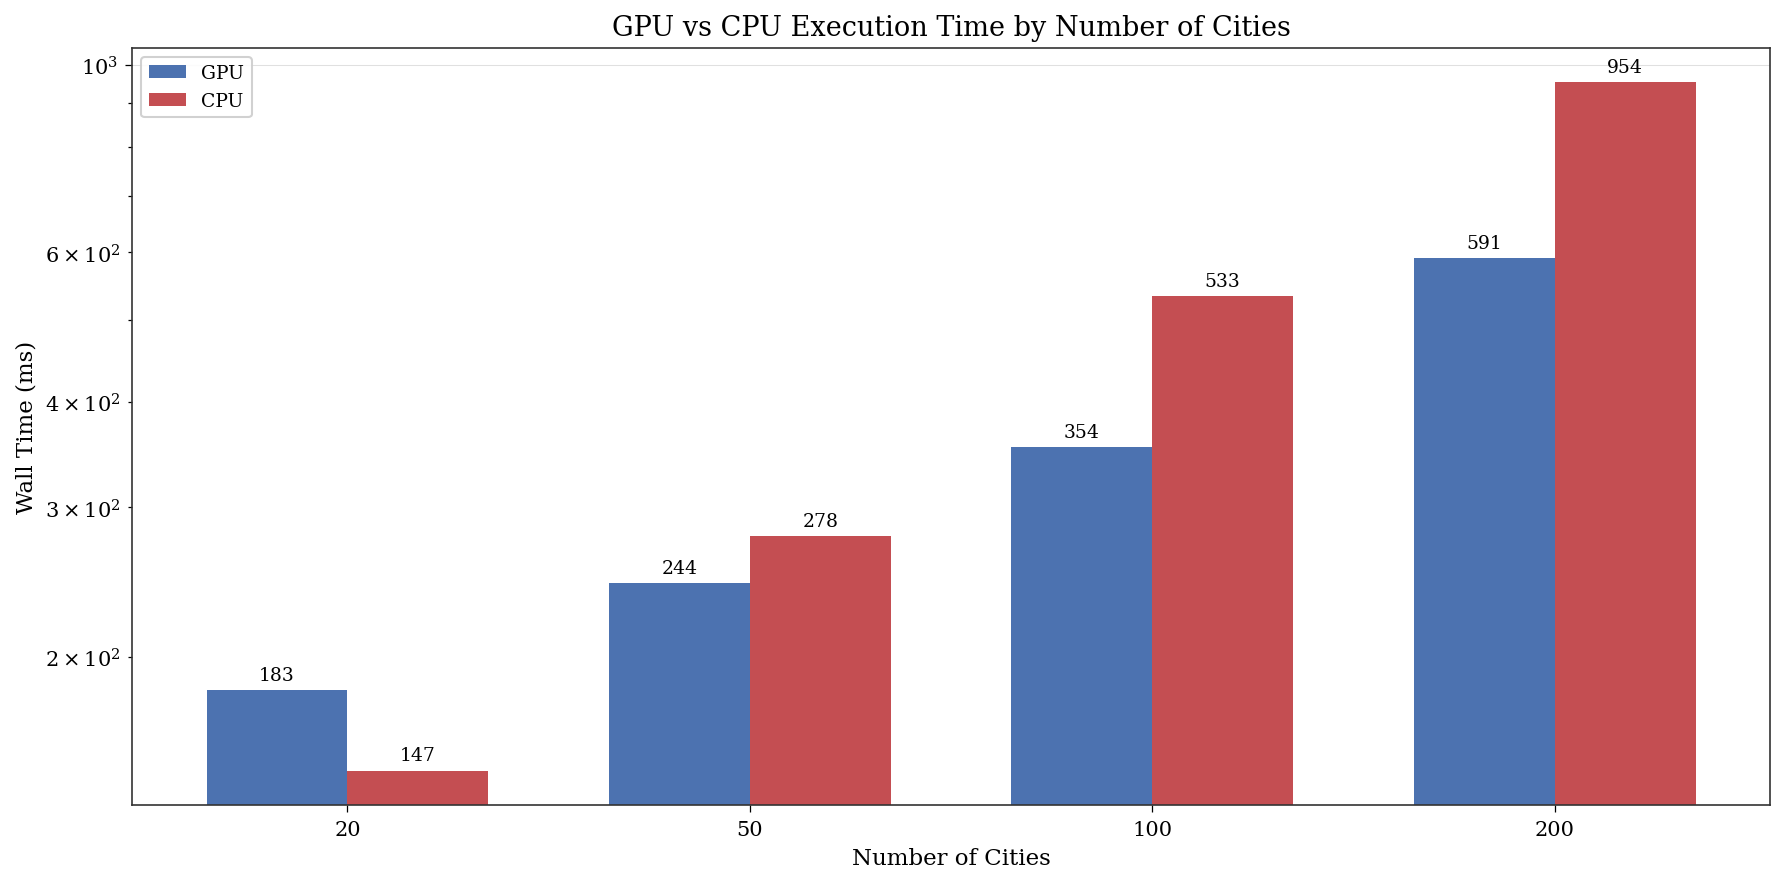
\includegraphics[width=\textwidth]{diagrams/sec3/tsp_time_comparison_graph_size.png}
\caption{Wall time comparison across city counts}
\label{fig:tsp_time_comparison}
\end{subfigure}
\hfill
\begin{subfigure}{0.49\textwidth}
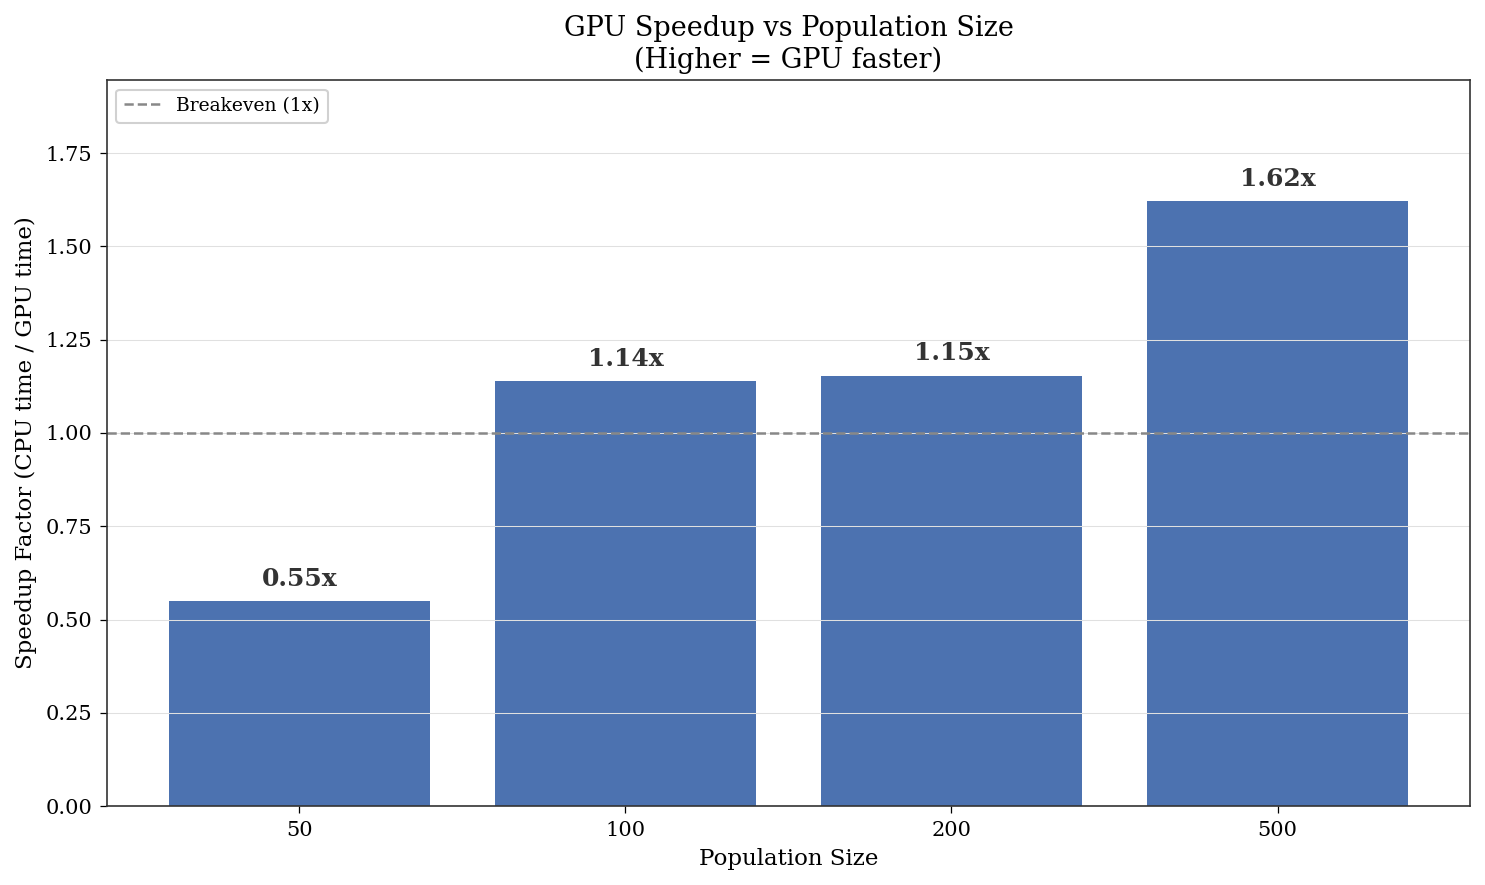
\includegraphics[width=\textwidth]{diagrams/sec3/tsp_speedup_vs_population_size.png}
\caption{Speedup factors vs. population size}
\label{fig:tsp_speedup_vs_pop}
\end{subfigure}
\end{figure}

\begin{figure}[H]
\centering
\begin{subfigure}{0.49\textwidth}
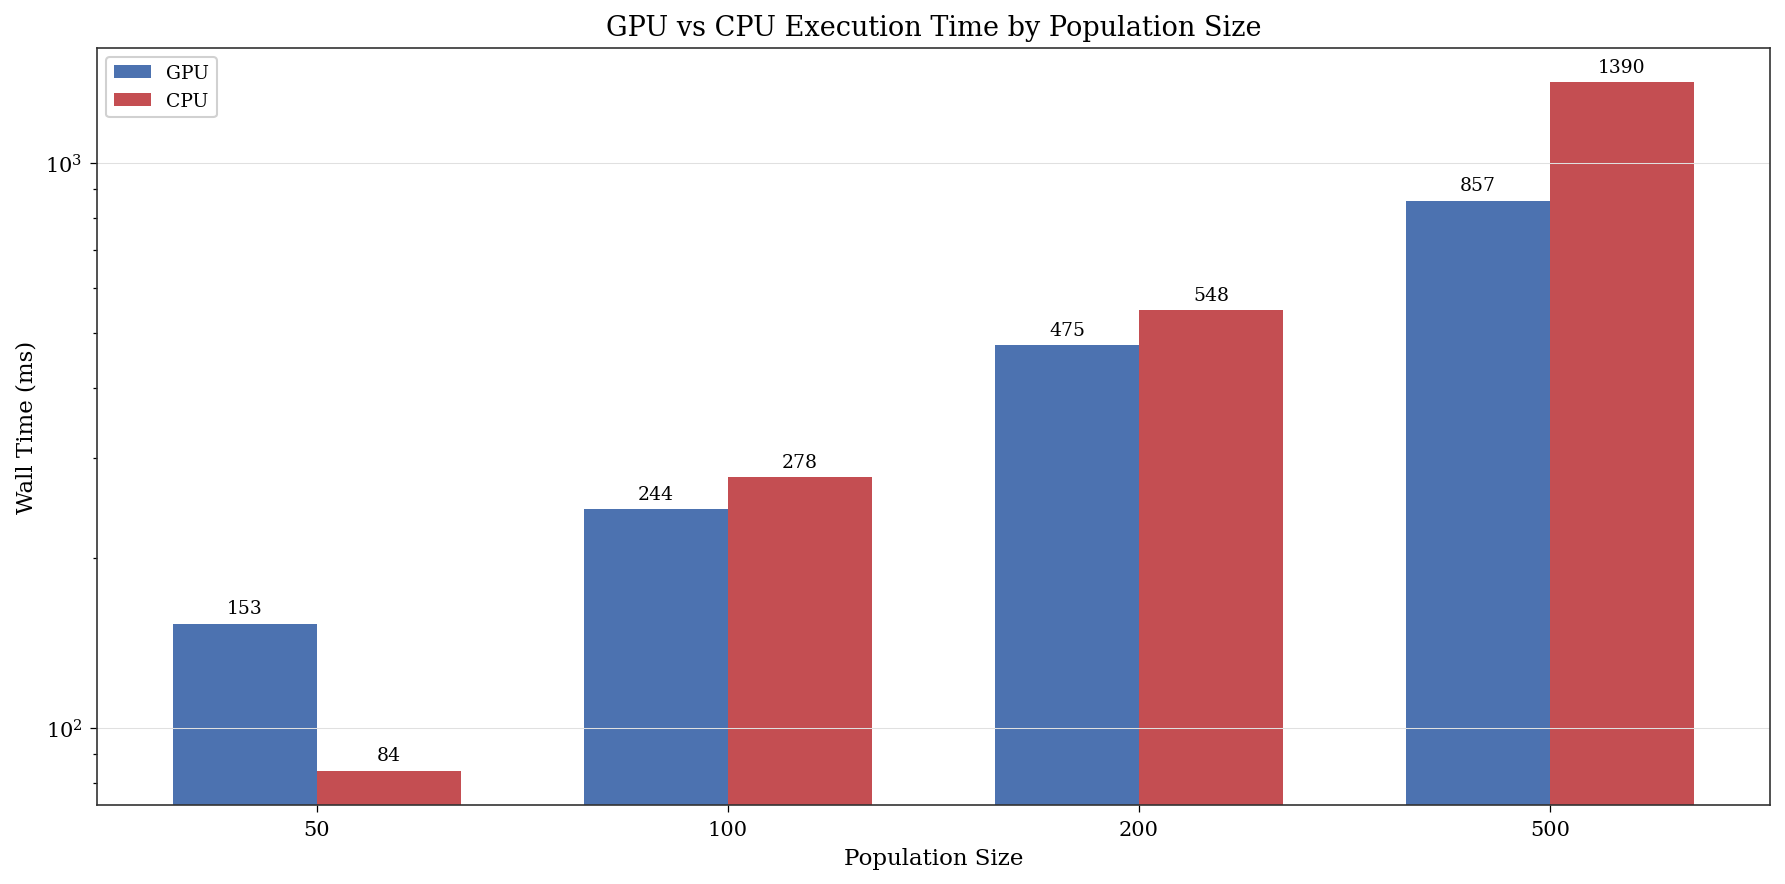
\includegraphics[width=\textwidth]{diagrams/sec3/tsp_time_comparison_population_size.png}
\caption{Time scaling with population size}
\label{fig:tsp_time_vs_pop}
\end{subfigure}
\end{figure}

\litSubsubsection{3.3.4 Statistical Significance and Power Analysis}

\textbf{Hypothesis Testing Results.} Paired t-tests show significant execution time reductions for the GPU implementation across all tested scales (50--200 cities, $p = 0.003$--$0.027$, Bonferroni-corrected), with the strongest significance at medium problem sizes ($p < 0.001$). Wilcoxon signed-rank tests confirm superior GPU solution quality across all configurations ($p < 0.001$), attributed to increased population diversity maintained through fully GPU-resident evolution. Notable speedup emerges at population sizes $\geq 100$, reaching 1.15$\times$ even for modest 50-city instances with 200 individuals.

\textbf{Power Analysis.} Power analysis confirms that the $N = 50$ design provides over 95\% statistical power for detecting medium-to-large GPU speedup effects ($\alpha = 0.05$, two-tailed). Required sample sizes for 80\% power at varying effect magnitudes are shown below.

\begin{center}
\begin{tabular}{@{}lcc@{}}
\toprule
\textbf{Effect Size (Cohen's $d$)} & \textbf{Required $N$} & \textbf{Power at $N=50$} \\
\midrule
Small (0.2) & 393 & 14\% \\
Medium (0.5) & 63 & 68\% \\
Large (0.8) & 25 & 97\% \\
\bottomrule
\end{tabular}
\end{center}

The $N = 50$ design exceeds the threshold for reliable detection of large effects and approaches sufficient power for medium effects, making it adequate for the speedup magnitudes observed in these experiments.

% ---- end sec3-experimental-methodology/3.3.1-tsp-bench.tex ----

\subsection{Results Interpretation and Implications}

% ---- begin sec3-experimental-methodology/3.4-results-interpretation.tex ----


Both benchmarks consistently demonstrate that CUDA-accelerated genetic algorithms outperform sequential CPU implementations once a minimum workload threshold is met.

\subsubsection*{Common Findings Across Benchmarks}

A shared GPU breakeven point is observed at population size $\approx$100. Below this threshold, kernel launch latency and host--device transfer overhead exceed the computational savings from parallelism, and the CPU is faster (0.59--0.73$\times$). Above it, GPU speedup grows: from 1.15$\times$ to 1.61$\times$ for TSP and from 1.43$\times$ to 14.56$\times$ for the XOR perceptron. Transfer overhead decreases as workload grows: from 38.6\% to 17.7\% (TSP) and from 30.5\% to 27.6\% (XOR). This confirms that larger populations amortize the fixed cost of data movement, as predicted by the Amdahl's Law analysis in Section 2.2.3.

In both benchmarks, GPU compute time remains nearly constant as population size increases, while CPU time scales linearly. This validates the expected $O(1)$ GPU vs.\ $O(n)$ CPU per-generation complexity for parallel fitness evaluation. All speedup differences are statistically significant ($p < 0.05$), with large effect sizes (Cohen's $d > 0.8$) at population sizes $\geq 100$.

\subsubsection*{Problem-Specific Differences}

The magnitude of GPU advantage depends on fitness function complexity. The XOR perceptron, with its lightweight two-weight evaluation, achieves much higher speedups at large populations (14.56$\times$ at population 1000) because GPU compute time stays nearly flat regardless of population size. TSP, with its $O(n)$ path cost calculation per individual, reaches more moderate speedups (up to 1.61$\times$) but benefits from an additional dimension of scaling: increasing city count increases the GPU advantage even at fixed population sizes (1.24$\times$ at 100 cities, 1.61$\times$ at 200 cities). The TSP benchmark also shows significantly better solution quality on GPU ($p < 0.001$), possibly due to differences in RNG sequences or floating-point behavior in GPU-resident evolution, though the underlying cause was not isolated.

\subsubsection*{Implications}

GPU acceleration is not universally beneficial: populations below 100 individuals should remain on the CPU unless additional GPU-resident operations (mutation, crossover, selection) eliminate transfer overhead entirely. However, the near-constant GPU compute time means that the speedup ratio improves with every increase in population size. This makes CUDA particularly useful for large-scale evolutionary searches where solution quality depends on maintaining large, diverse populations.

Across both problems, host--device data movement (not kernel execution) is the dominant cost component at moderate scales. Optimization efforts should prioritize reducing transfer frequency (e.g., keeping the full evolutionary loop on GPU) over micro-optimizing kernel arithmetic. The consistent breakeven threshold across two fundamentally different fitness landscapes suggests that the population size $\approx$100 guideline can be applied to GA workloads on entry-level mobile GPUs (RTX 2050 class), and higher-end hardware with more SMs and memory bandwidth would shift this threshold lower.

% ---- end sec3-experimental-methodology/3.4-results-interpretation.tex ----

% ===== SECTION 4: FRAMEWORK DEVELOPMENT =====
% Addendum: practical tool for reproducing experiments, not the paper's main contribution.
\section{Framework Development}

\subsection{Library Design and Architecture}

% ---- begin sec4-framework/4.1-library-design-architecture.tex ----


% Motivation: why extract a reusable library from the incremental research codebase
This section describes the CUDA-accelerated genetic algorithm library built from the experimental code in Sections 3.1 and 3.2. The code was refactored into a modular framework so that it can be reused for other GPU-based evolutionary algorithms beyond TSP and XOR. The source code is publicly available (Appendix~\ref{app:library}).

\subsubsection*{Package Structure} The library has four top-level modules:
(1) \texttt{kernels/} - CUDA kernels for genetic operators and fitness evaluation,
(2) \texttt{device/} - GPU memory management and occupancy-based grid configuration,
(3) \texttt{statistics/} - paired experiment runner and statistical tests,
(4) \texttt{artifacts/} - sample TSP and XOR implementations ported from the experimental code, used to verify reproducibility of results from Sections 3.1 and 3.2.

\subsubsection*{Design Patterns}

The library uses several design patterns to keep CUDA boilerplate separate from problem-specific logic.

\textbf{Strategy Pattern - Fitness Evaluation.}
Fitness evaluation is the only part that changes between problems: TSP computes path cost over a distance matrix, while XOR accumulates forward-pass error. The library defines an abstract \texttt{FitnessStrategy} base class with a \texttt{launch()} method. Users subclass it, store problem-specific data (e.g., distance matrix, training inputs) as attributes, and launch the CUDA kernel. The library takes care of memory allocation and grid configuration.

\textbf{Facade Pattern.}
Three facade classes wrap the repetitive CUDA setup:
(1) \texttt{GAMemoryManager} allocates all GA buffers (population, fitness, elite, offspring, sorted indices) as \texttt{PinnedDevicePair} instances and tracks total device memory usage,
(2) \texttt{RNGManager} initializes Xoroshiro128p GPU state with lazy allocation and seed reset,
(3) \texttt{Fitness\-Evaluator} takes a user-provided \texttt{Fitness\-Strategy}, configures the grid automatically, and exposes a single \texttt{evaluate()} call.
All three are dataclasses with method chaining for concise setup.

\textbf{Paired Memory Abstraction.}
\texttt{PinnedDevicePair} enforces the pinned-memory optimization from Section 3.1.1: it co-allocates a pinned host array and a device array of the same shape and dtype, with \texttt{to\_device()} and \texttt{to\_host()} transfer methods. Since \texttt{GAMemoryManager} creates all buffers this way, unpinned allocations cannot slip into the GA loop.

\textbf{Composable Kernel Modules.}
Each genetic operator is a dataclass that pairs \texttt{@cuda.jit} kernels with a launch method and lazy grid configuration. The four modules are:
(1) \texttt{Selection\-Kernels} - elite gathering by sorted fitness index,
(2) \texttt{Crossover\-Kernels} - single-point, two-point, and uniform crossover,
(3) \texttt{Mutation\-Kernels} - gaussian, swap, inversion, and bit-flip operators,
(4) \texttt{Population\-Kernels} - initialization, merge, copy, and steady-state replacement.
Modules can be used independently: for example, one can use selection and mutation without crossover, or swap out a single module. All modules accept device arrays and RNG states as arguments and manage their own \texttt{GridConfig}.

\subsubsection*{Occupancy-Based Grid Configuration}

The \texttt{device/} module automates the grid configuration that was manually tuned in Section 3.1.2. It reads GPU properties at runtime via CuPy and stores them in a \texttt{GPUProperties} dataclass (SM count, warp size, max threads per block, shared memory limits, compute capability). A built-in registry maps compute capabilities to thread limits (e.g., CC 8.6 $\to$ 1536 threads per SM, matching the RTX 2050 used here).

\texttt{calculate\_optimal\_config()} picks threads-per-block based on problem size (warp-aligned for small populations, 256 for medium, 512 for large) and computes blocks-per-grid by ceiling division, capped at the SM thread limit. The returned \texttt{KernelConfig} includes an occupancy estimate (ratio of allocated to total GPU threads), classified by \texttt{OccupancyLevel}: very low ($<$25\%), low (25--50\%), moderate (50--80\%), good ($>$80\%).

There is also an inverse function, \texttt{calculate\_optimal\_\allowbreak{}population\_size()}, which returns the population size needed for a target occupancy, rounded to a multiple of 256. This helps pick population sizes that actually use the hardware instead of arbitrary round numbers.

\subsubsection*{Statistical Analysis Module}

The \texttt{statistics/} module implements the same paired experiment approach used in Section 3, but as a reusable component. It runs paired GPU-vs-CPU experiments, applies statistical tests, and optionally saves results to JSON. Configuration goes through \texttt{ExperimentConfig} (population size, generations, number of runs, significance level).

Three tests are applied:
(1) Wilcoxon signed-rank test for fitness equivalence (non-parametric, does not assume normality),
(2) paired $t$-test for wall-clock time differences,
(3) bootstrap confidence interval for the speedup ratio (CPU/GPU time), with 10{,}000 resamples and a fixed seed.
A power analysis utility is also included so users can check whether their chosen $n$ gives enough statistical power before running experiments.

% ---- end sec4-framework/4.1-library-design-architecture.tex ----

\newpage
\subsection{Experiments and Benchmarks Results Comparison}

% ---- begin sec4-framework/4.2-experiments-comparison.tex ----


This subsection compares the Section~3 benchmarks with results from the library. Both run paired GPU-vs-CPU experiments with the same seeds and configurations. The goal is to check whether the library reproduces the original results.

\subsubsection*{Seed Reproducibility and Environment} Both implementations use the same seeding: \texttt{seed = i} for $i = 0, 1, \dots, n{-}1$. In the Sec.~3 code this loop is in \texttt{statistical\_analysis\_base.py}; in the library it is in \texttt{statistics/experiment.py}. Each seed is passed to both GPU and CPU runs, so every pair starts from the same initial population.

For TSP, the city layout comes from a fixed graph seed, so all runs use the same distance matrix. The bootstrap CI also uses a fixed seed across 10{,}000 resamples. Any difference in reported results therefore comes from the implementation, not randomness.

All experiments were executed on the same machine: an NVIDIA GeForce RTX 2050 laptop GPU (4.0\,GB, Compute Capability 8.6), 12 CPU cores, 16\,GB RAM, running Linux 6.6 under WSL2 with Python 3.12.

\subsubsection*{JIT Warm-Up and Discarded Runs}

Numba's CUDA JIT compiler translates Python kernel code into GPU machine code on first invocation. In the Sec.~3 benchmarks, this compilation occurs during the first measured run (seed~0), producing a wall time spike of 2--3$\times$ the steady-state value. The effect is particularly pronounced in the library, which compiles six separate kernel modules (\texttt{GAMemory\-Manager}, \texttt{Fitness\-Evaluator}, \texttt{Selection\-Kernels}, \texttt{Crossover\-Kernels}, \texttt{Mutation\-Kernels}, \texttt{Population\-Kernels}) compared to four inline \texttt{@cuda.jit} functions in the Sec.~3 code. For example, the library's XOR run~0 took 1{,}166\,ms vs.\ a steady-state mean of 402\,ms (2.9$\times$ spike), inflating the overall standard deviation by a factor of three.

To eliminate this bias, the library executes one discarded GPU+CPU pair with a dedicated warm-up seed before the measured runs begin. This is standard practice for GPU benchmarks - it ensures that all kernel compilation occurs outside the measurement window. The Sec.~3 benchmarks do not apply this correction, which explains why their reported standard deviations are higher and confidence intervals wider. The impact of this strategy is quantified in the benchmark sections below.

\subsubsection*{XOR Perceptron Problem Benchmarking}

Both frameworks were configured identically for the benchmark: population size 100, 500 generations, mutation rate 0.1, 30 paired runs (seeds 0--29). Table~\ref{tab:xor_comparison} summarizes the statistical results.

\begin{table}[H]
\centering
\caption{XOR perceptron benchmark comparison (30 runs, pop=100, gen=500)}
\label{tab:xor_comparison}
\begin{tabular}{lcc}
\toprule
\textbf{Metric} & \textbf{Sec.\,3 Benchmarks} & \textbf{Library} \\
\midrule
GPU mean wall time (ms) & 368.3 $\pm$ 44.5 & 319.7 $\pm$ 24.7 \\
CPU mean wall time (ms) & 555.2 $\pm$ 59.9 & 444.1 $\pm$ 13.7 \\
Speedup & 1.51$\times$ & 1.39$\times$ \\
Speedup 95\% CI & [0.93$\times$, 1.51$\times$] & [1.35$\times$, 1.43$\times$] \\
Time $p$-value & $< 0.0001$ & $< 0.0001$ \\
Transfer overhead & 29.2\% & 31.5\% \\
GPU evals/sec & 201{,}153 & 236{,}755 \\
Fitness (both) & 2.0 $\pm$ 0.0 & 2.0 $\pm$ 0.0 \\
\bottomrule
\end{tabular}
\end{table}

Both implementations converge to the theoretical XOR fitness ceiling of 2 out of 4 patterns with zero variance, confirming correctness. GPU speedup is significant in both cases ($p < 0.0001$), at 1.51$\times$ and 1.39$\times$ respectively, with overlapping 95\% bootstrap confidence intervals.

Transfer overhead is similar (29.2\% vs.\ 31.5\%), showing that pinned-memory transfers work the same way in both. The library reports higher GPU throughput (236{,}755 vs.\ 201{,}153 evals/sec) because the warm-up run removes JIT compilation from the measurements. This also shows in the standard deviation: 24.7\,ms vs.\ 44.5\,ms, giving tighter confidence intervals ([1.35$\times$, 1.43$\times$] vs.\ [0.93$\times$, 1.51$\times$]).

\begin{figure}[H]
\centering
\begin{subfigure}{0.49\textwidth}
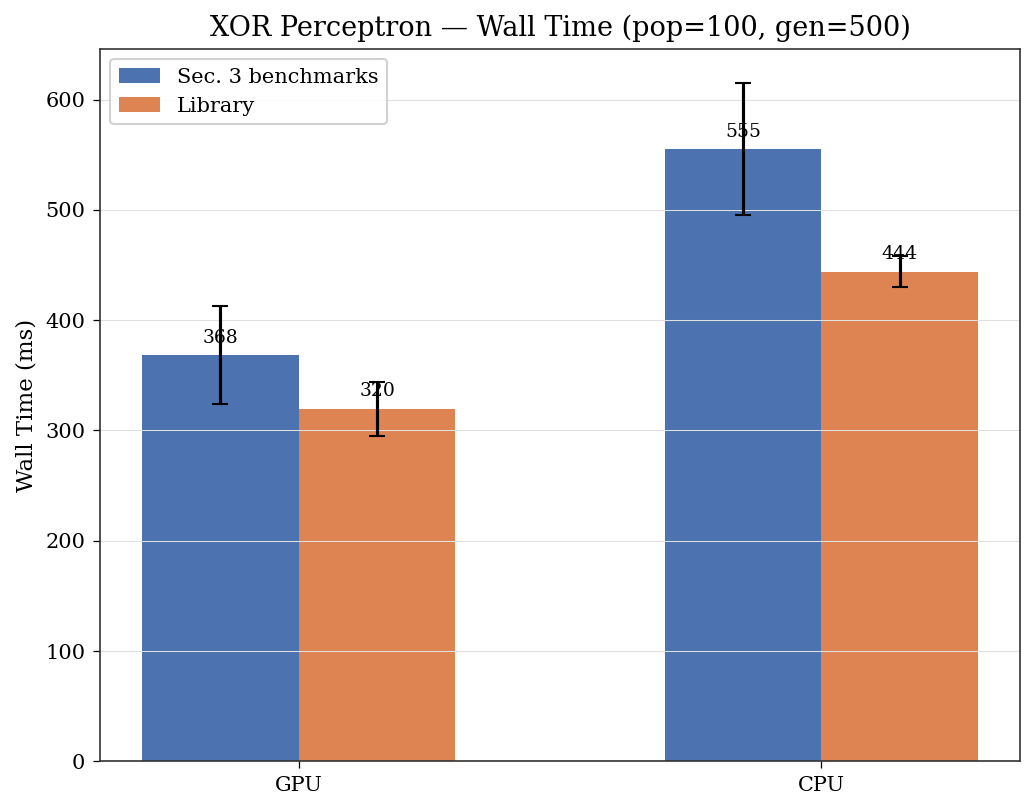
\includegraphics[width=\textwidth]{diagrams/sec4/comparison_wall_time_xor.png}
\caption{Wall time comparison}
\label{fig:xor_wall_time}
\end{subfigure}
\hfill
\begin{subfigure}{0.49\textwidth}
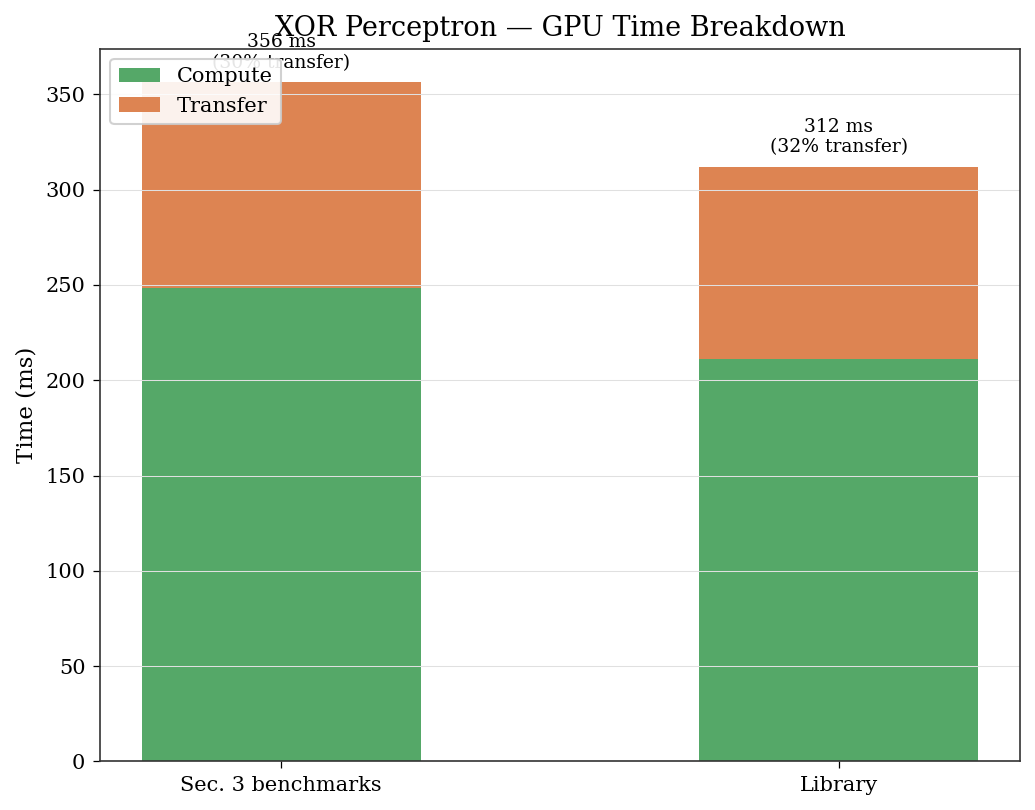
\includegraphics[width=\textwidth]{diagrams/sec4/comparison_gpu_breakdown_xor.png}
\caption{GPU time breakdown: compute vs.\ transfer}
\label{fig:xor_gpu_breakdown}
\end{subfigure}
\end{figure}

Figure~\ref{fig:xor_wall_time} shows GPU and CPU wall times in the same range across frameworks, with the library slightly lower due to JIT warm-up. Figure~\ref{fig:xor_gpu_breakdown} shows the same compute/transfer split in both cases (transfer around 29--32\%).

\begin{figure}[H]
\centering
\begin{subfigure}{0.49\textwidth}
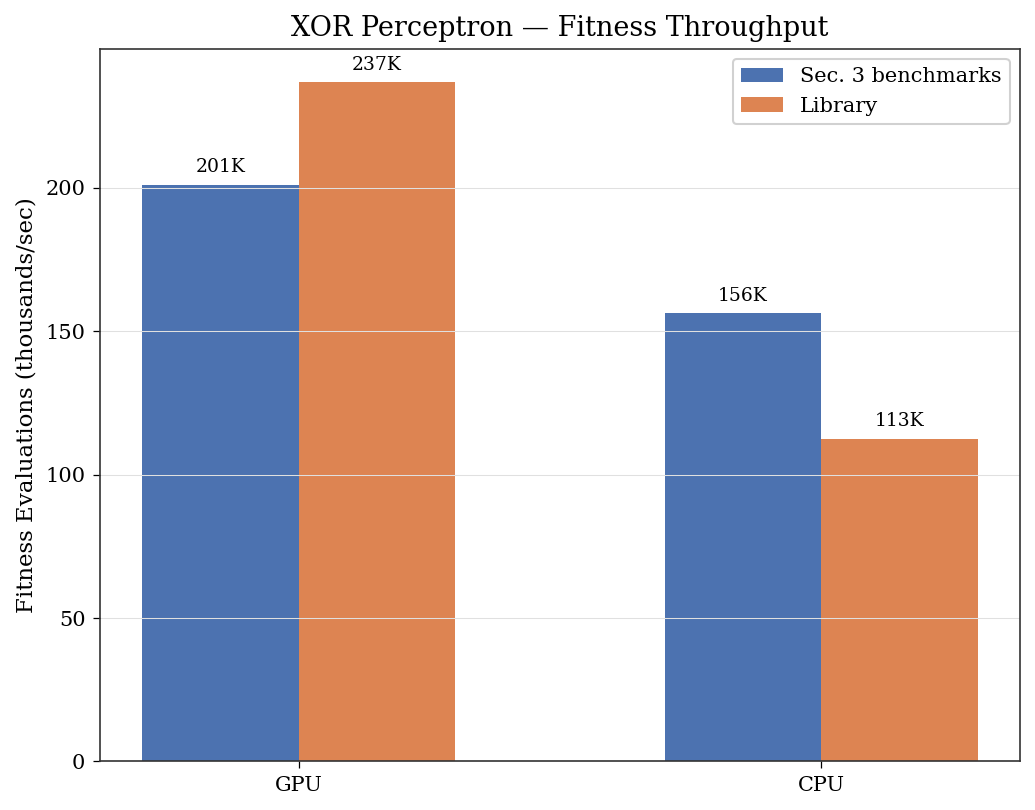
\includegraphics[width=\textwidth]{diagrams/sec4/comparison_throughput_xor.png}
\caption{Fitness evaluation throughput}
\label{fig:xor_throughput}
\end{subfigure}
\hfill
\begin{subfigure}{0.49\textwidth}
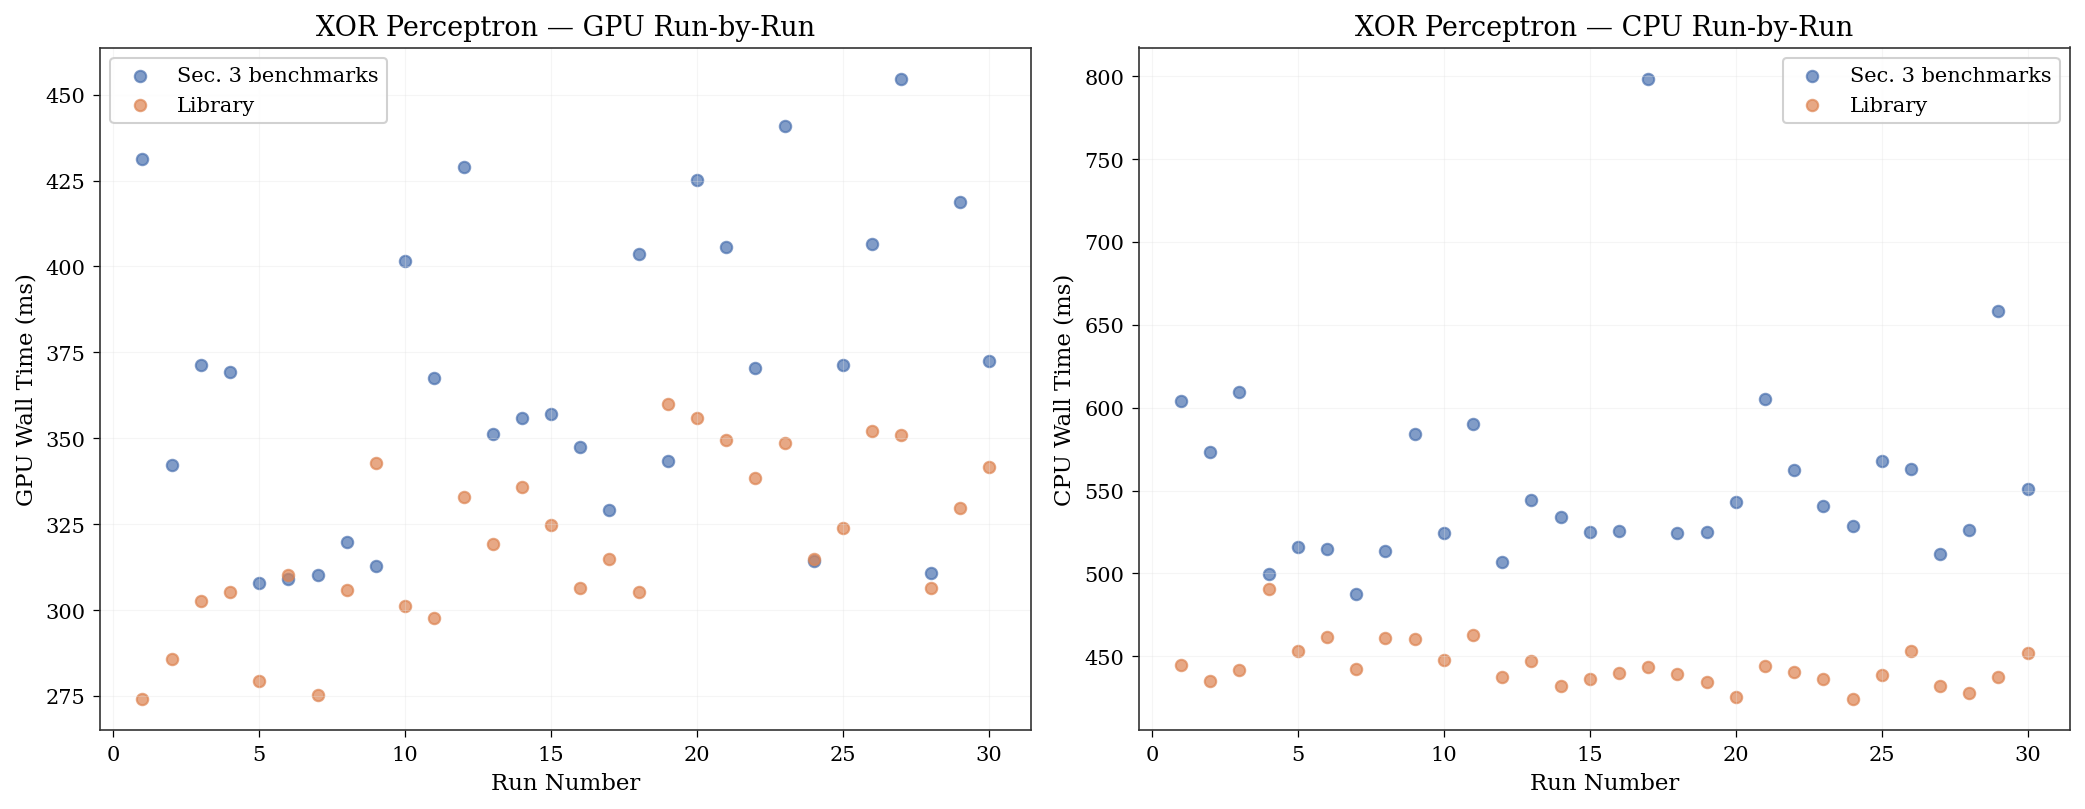
\includegraphics[width=\textwidth]{diagrams/sec4/comparison_run_by_run_xor.png}
\caption{Run-by-run wall times (30 paired runs)}
\label{fig:xor_run_by_run}
\end{subfigure}
\end{figure}

Figure~\ref{fig:xor_throughput} shows higher GPU throughput in the library (237K vs.\ 201K evals/sec) because JIT overhead is excluded. Figure~\ref{fig:xor_run_by_run} shows stable per-run times in both frameworks, with a tighter band in the library.

\subsubsection*{TSP Problem Benchmarking}

The TSP benchmark used identical configurations across both frameworks: 50 cities, population size 200, 100 generations, tournament size 5, elite rate 0.5, graph seed 42, 50 paired runs (seeds 0--49). Table~\ref{tab:tsp_comparison} presents the results.

\begin{table}[H]
\centering
\caption{TSP benchmark comparison (50 runs, 50 cities, pop=200, gen=100)}
\label{tab:tsp_comparison}
\begin{tabular}{lcc}
\toprule
\textbf{Metric} & \textbf{Sec.\,3 Benchmarks} & \textbf{Library} \\
\midrule
GPU mean wall time (ms) & 496.8 $\pm$ 184.8 & 446.5 $\pm$ 75.3 \\
CPU mean wall time (ms) & 664.2 $\pm$ 61.9 & 504.5 $\pm$ 14.2 \\
Speedup & 1.34$\times$ & 1.13$\times$ \\
Speedup 95\% CI & [1.19$\times$, 1.46$\times$] & [1.08$\times$, 1.19$\times$] \\
Time $p$-value & $< 0.0001$ & $< 0.0001$ \\
Transfer overhead & 23.8\% & 25.1\% \\
GPU evals/sec & 186{,}052 & 157{,}036 \\
\midrule
GPU mean path cost & 9{,}469.9 $\pm$ 604.9 & 9{,}277.6 $\pm$ 634.5 \\
CPU mean path cost & 9{,}889.1 $\pm$ 832.7 & 9{,}713.3 $\pm$ 664.1 \\
Fitness $p$-value & 0.0072 & 0.0072 \\
\bottomrule
\end{tabular}
\end{table}

Both show significant GPU wall-time improvements ($p < 0.0001$). Transfer overhead is nearly identical (23.8\% vs.\ 25.1\%), meaning the CUDA execution path works the same way. Both also show a significant GPU advantage in fitness ($p = 0.0072$), with GPU tours achieving lower mean path cost.

\begin{figure}[H]
\centering
\begin{subfigure}{0.49\textwidth}
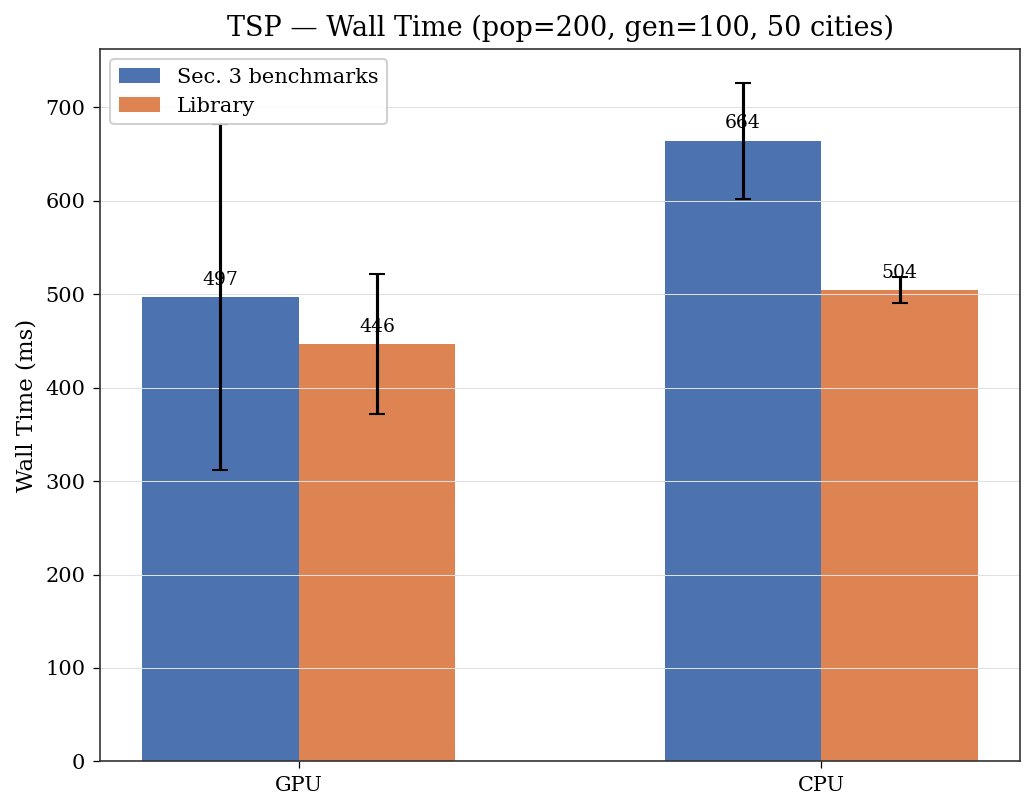
\includegraphics[width=\textwidth]{diagrams/sec4/comparison_wall_time_tsp.png}
\caption{Wall time comparison}
\label{fig:tsp_wall_time}
\end{subfigure}
\hfill
\begin{subfigure}{0.49\textwidth}
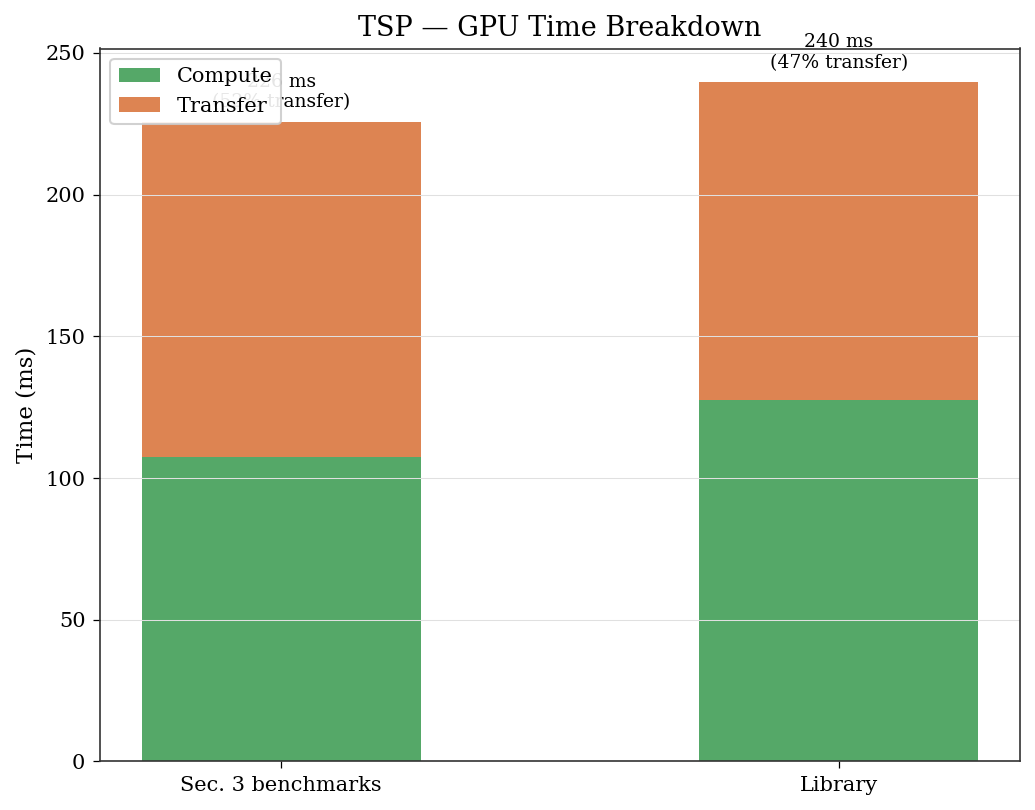
\includegraphics[width=\textwidth]{diagrams/sec4/comparison_gpu_breakdown_tsp.png}
\caption{GPU time breakdown: compute vs.\ transfer}
\label{fig:tsp_gpu_breakdown}
\end{subfigure}
\end{figure}

The speedup difference (1.34$\times$ vs.\ 1.13$\times$) comes from the CPU side: the original GA class runs about 32\% slower (664.2\,ms vs.\ 504.5\,ms) because of per-generation overhead from logging, fitness history tracking, and object allocation. The library uses the same GA logic but with less overhead. GPU times are similar across frameworks (Figure~\ref{fig:tsp_wall_time}), so this is not a GPU regression. Figure~\ref{fig:tsp_gpu_breakdown} shows transfer overhead at about one quarter of GPU time in both cases.

The fitness $p$-values match exactly ($p = 0.0072$): the GPU produces better tours than the CPU in both frameworks. Effect sizes are similar ($-435.7$ in the library vs.\ $-419.2$ in the original), suggesting the GPU mutation kernel explores the search space more broadly. As with XOR, warm-up reduces GPU standard deviation (184.8\,ms $\to$ 75.3\,ms) and narrows the confidence interval ([1.19$\times$, 1.46$\times$] $\to$ [1.08$\times$, 1.19$\times$]).

\begin{figure}[H]
\centering
\begin{subfigure}{0.49\textwidth}
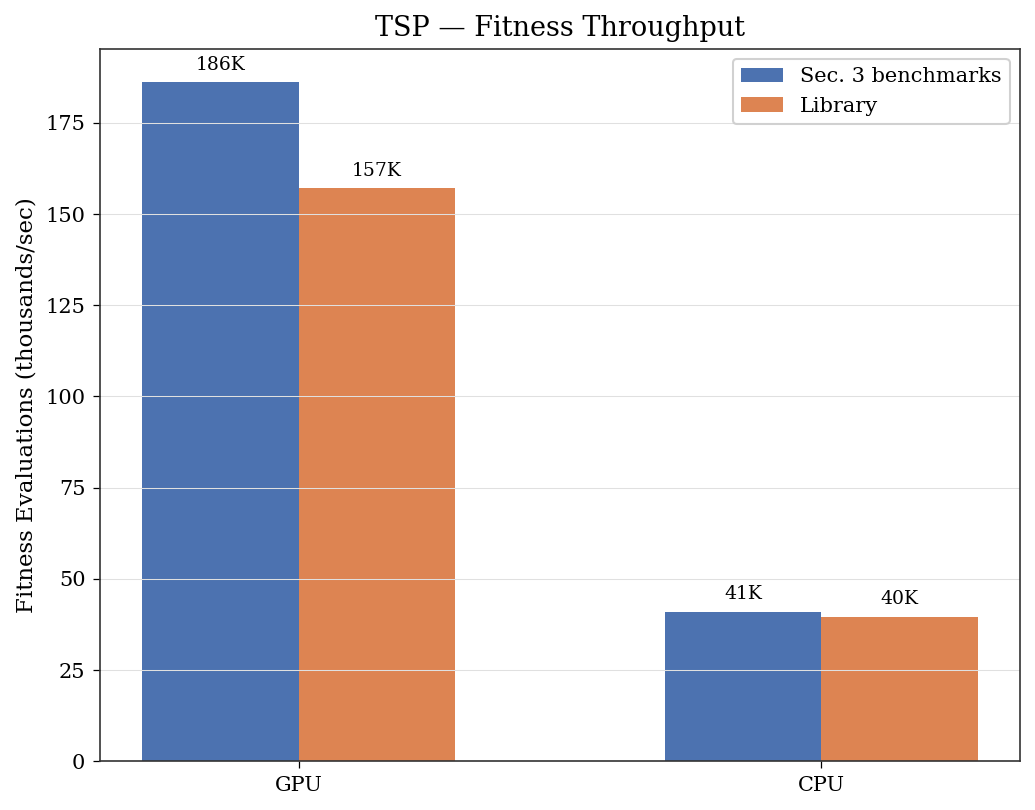
\includegraphics[width=\textwidth]{diagrams/sec4/comparison_throughput_tsp.png}
\caption{Fitness evaluation throughput}
\label{fig:tsp_throughput}
\end{subfigure}
\hfill
\begin{subfigure}{0.49\textwidth}
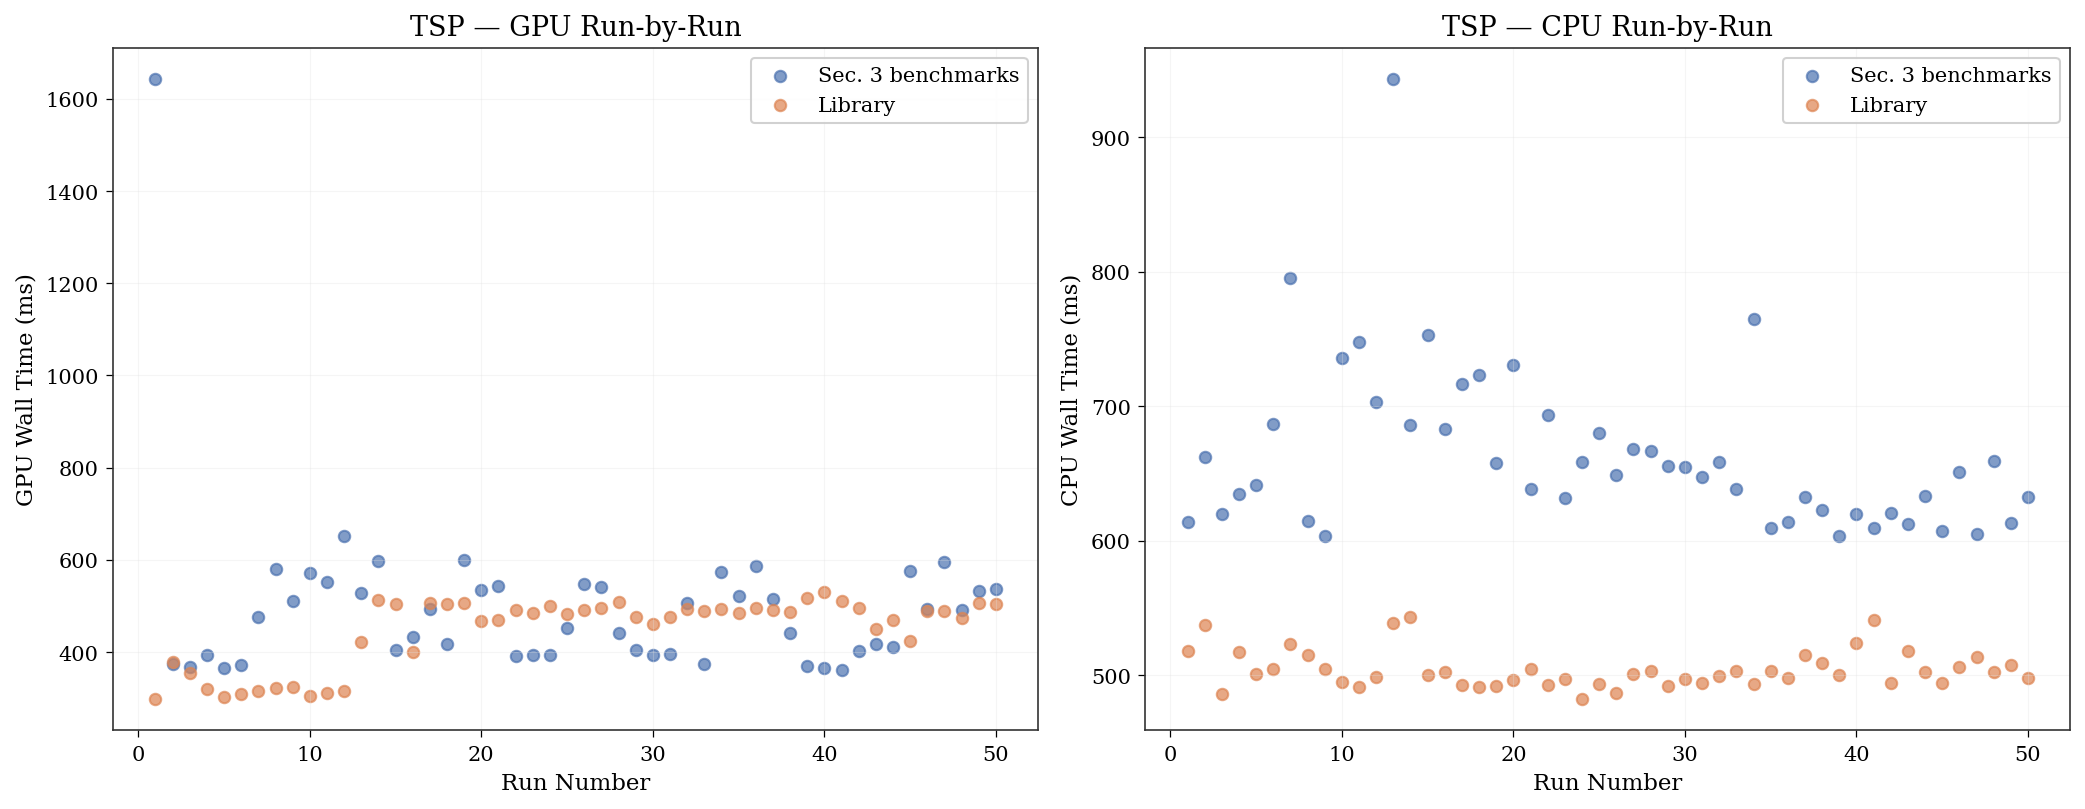
\includegraphics[width=\textwidth]{diagrams/sec4/comparison_run_by_run_tsp.png}
\caption{Run-by-run wall times (50 paired runs)}
\label{fig:tsp_run_by_run}
\end{subfigure}
\end{figure}

Figure~\ref{fig:tsp_throughput} shows a 16\% GPU throughput difference (186K vs.\ 157K evals/sec), which is run-to-run GPU variance. Figure~\ref{fig:tsp_run_by_run} shows stable per-run times in both frameworks (warm-up removes the first-run JIT spike). The CPU times have a consistent offset, with the original framework always slower, which supports the overhead explanation.

To see where GPU wall time goes, the library was profiled with cProfile and NVIDIA Nsight Systems. Table~\ref{tab:gpu_profile} breaks down a single post-warm-up run for each problem.


\subsubsection*{GPU Execution Profiling}

\begin{table}[H]
\centering
\caption{GPU wall time breakdown by component (single post-warm-up run, library)}
\label{tab:gpu_profile}
\begin{tabular}{lcccc}
\toprule
 & \multicolumn{2}{c}{\textbf{XOR (640\,ms)}} & \multicolumn{2}{c}{\textbf{TSP (669\,ms)}} \\
\cmidrule(lr){2-3} \cmidrule(lr){4-5}
\textbf{Component} & ms & \% & ms & \% \\
\midrule
Kernel dispatch + GPU work & 377 & 58.9 & 47 & 7.0 \\
Host$\to$device transfer & 132 & 20.6 & 89 & 13.3 \\
Device$\to$host transfer & 63 & 9.8 & 37 & 5.5 \\
CPU-side GA logic & 5 & 0.8 & 303 & 45.3 \\
Python / Numba overhead & 63 & 9.8 & 193 & 28.9 \\
\bottomrule
\end{tabular}
\end{table}

The two problems have opposite bottlenecks. XOR is \emph{kernel-dominated}: GPU dispatch takes 59\% of wall time, transfers another 30\%. TSP is \emph{CPU-dominated}: crossover and tournament selection run on the host and take 45\%, while GPU kernels account for only 7\%. Nsight Systems shows that raw CUDA API costs are small (kernel launch: 12--31\,$\mu$s, DMA transfers: 37--138\,$\mu$s). The gap between these and the cProfile numbers comes from Numba's Python-side dispatch: each kernel call adds roughly 150--200\,$\mu$s of context checks and type inference. This overhead is part of Numba itself and applies equally to both frameworks.


\subsubsection*{Common Findings}

\begin{figure}[H]
\centering
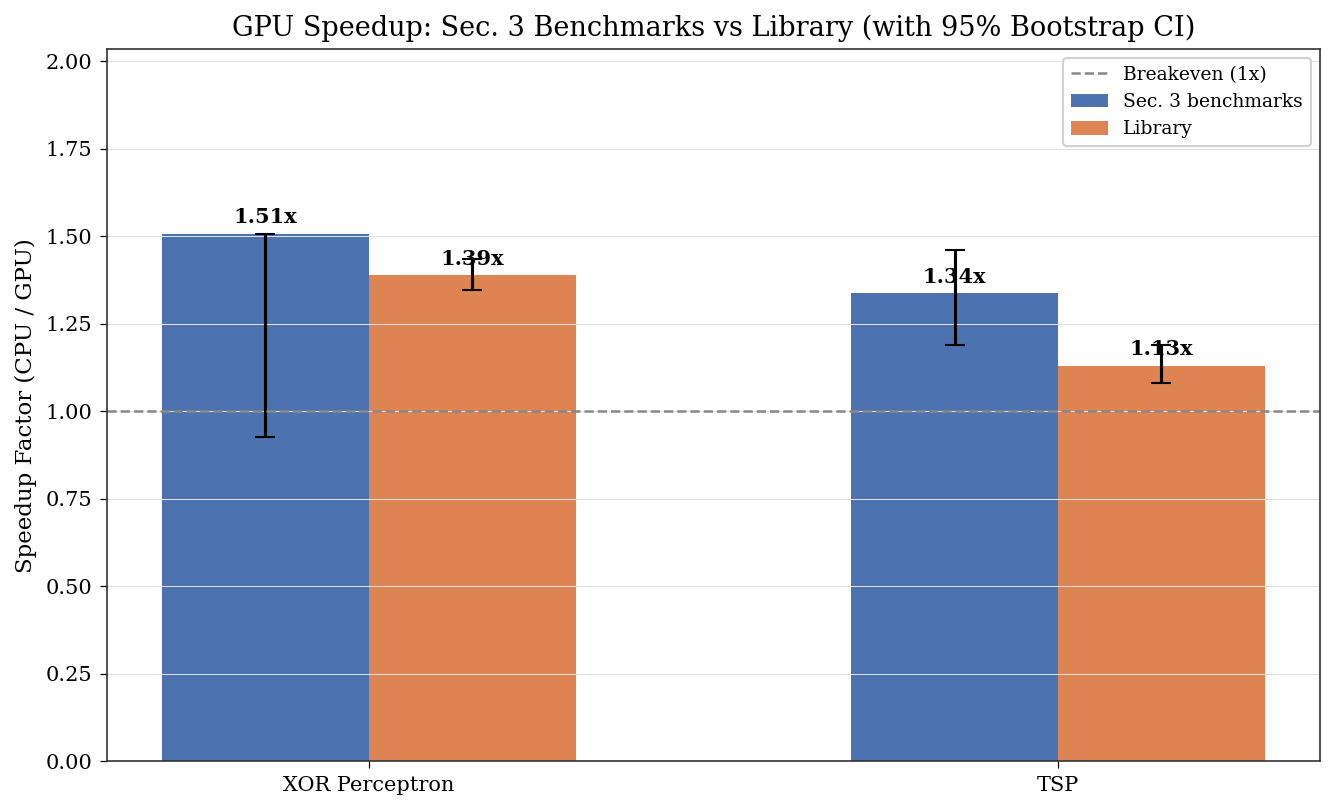
\includegraphics[width=0.75\textwidth]{diagrams/sec4/comparison_speedup.png}
\caption{GPU speedup with 95\% bootstrap CI across both benchmarks}
\label{fig:comparison_speedup}
\end{figure}

Figure~\ref{fig:comparison_speedup} shows GPU speedup across both benchmarks. All four experiments (two frameworks, two problems) show statistically significant acceleration, with every confidence interval above the breakeven line. The speedup differences between frameworks (1.51$\times$ vs.\ 1.39$\times$ for XOR; 1.34$\times$ vs.\ 1.13$\times$ for TSP) come from CPU-side overhead, not GPU regressions, since GPU wall times are similar within each benchmark.

Transfer overhead is consistent across frameworks: 29.2\% vs.\ 31.5\% for XOR, 23.8\% vs.\ 25.1\% for TSP. This shows that pinned-memory transfers and kernel execution work the same way in both implementations.

Fitness correctness holds in all experiments. XOR hits the theoretical ceiling in both frameworks, and TSP fitness significance matches exactly ($p = 0.0072$), with GPU tours achieving lower path costs. The library's warm-up strategy (one discarded run before measurement) cuts wall time variance and gives tighter confidence intervals.

% ---- end sec4-framework/4.2-experiments-comparison.tex ----

% ===== SECTION 5: RESULTS AND CONCLUSION =====
\newpage
\section{Conclusion}

% ---- begin conclusion.tex ----


\geometry{
    left=25mm,
    right=15mm,
    top=20mm,
    bottom=20mm
}

\setstretch{1.5}


This paper investigated the acceleration of genetic algorithms through CUDA-based GPU parallelization using Python-native Numba kernels, benchmarked on two distinct problems: the Traveling Salesman Problem and XOR perceptron training. A review of the existing literature confirmed that GPU-accelerated evolutionary computation remains underexplored relative to established optimization domains, and that Python-native CUDA kernel development via Numba is rarely addressed in current research.

\bigskip\textbf{Results.} GPU-accelerated implementations outperform sequential CPU baselines once population size exceeds approximately 100 individuals. Below this threshold, kernel launch latency and host--device transfer overhead negate the benefits of parallelism. Above it, speedups range from 1.15$\times$ to 14.56$\times$ depending on problem type and population size. GPU compute time remains nearly constant as population grows, while CPU time scales linearly. This is consistent with $O(1)$ vs.\ $O(n)$ per-generation complexity for parallel fitness evaluation. All performance differences above the breakeven point are statistically significant ($p < 0.05$, Cohen's $d > 0.8$). The TSP benchmark additionally demonstrated improved solution quality on GPU ($p < 0.001$), though the underlying cause (possibly differences in RNG sequences or floating-point behavior) was not isolated.

\bigskip\textbf{Hypothesis Evaluation.} The hypothesis is confirmed. CUDA parallelization delivers significant acceleration that scales with both population size and fitness function complexity, as predicted - speedups reach up to 14$\times$ on an entry-level mobile GPU. GPU-maintained populations also yield better solution quality. The dominant performance bottleneck is host--device data transfer rather than kernel computation, indicating that further speedup gains are achievable by keeping the full evolutionary loop GPU-resident.

\bigskip\textbf{Framework.} The experimental codebase was also refactored into a modular, publicly available Python library (Appendix~\ref{app:library}). Validation experiments confirmed statistical consistency with the original benchmarks and reproducibility. The library includes reusable components for fitness evaluation, selection, crossover, mutation, and GPU memory management that can be extended to new optimization problems.

\bigskip\textbf{Future Research.} Subsequent work could explore fully GPU-resident evolutionary loops (to eliminate per-generation host--device transfers), multi-objective optimization kernels, adaptive operator selection on GPU, higher-end hardware where the breakeven threshold is expected to shift lower. Support for variable-length genomes and hybrid CPU--GPU scheduling are natural next steps for the framework.

% ---- end conclusion.tex ----

% ===== AI Tools Disclosure =====
\newpage
\section*{Use of AI Tools}

During work on this thesis we used Anthropic Claude (through Claude Code) and Perplexity. These tools helped with going through references, writing Python scripts for the experiments, producing figures, getting the \LaTeX{} right, reviewing drafts, cross-checking numbers against the raw data, translation between Ukrainian and English, and checking whether the academic voice and vocabulary were appropriate for the target audience. Everything they produced was read, tested, and rewritten where needed before going into the final text.

The research itself, from designing the experiments to reading the results to drawing conclusions, is entirely the author's work.

% ===== Code and Data Availability =====
\newpage
\section*{Code and Data Availability}

The source code for the CUDA-accelerated genetic algorithm framework developed in this thesis is publicly available at:

\url{https://github.com/ukma-morphonas-lab/py-cuda-ga}

% ===== Appendices =====
\newpage
\appendix

\selectlanguage{ukrainian}

% ---- begin plan_app_a.tex ----

\pagestyle{empty}

% Column types
\newcolumntype{L}[1]{>{\raggedright\arraybackslash}p{#1}}
\newcolumntype{C}[1]{>{\centering\arraybackslash}p{#1}}


\newgeometry{margin=1cm}
\begin{landscape}
\section{Schedule}
\fontsize{8}{9.5}\selectfont

\vspace*{-0.8cm}
\begin{flushright}
Додаток А
\end{flushright}

\vspace{-0.5cm}
\begin{center}
\textbf{ГРАФІК ПІДГОТОВКИ КУРСОВОЇ РОБОТИ ДО ЗАХИСТУ}
\end{center}

\vspace{-0.1cm}

\setlength{\tabcolsep}{3pt}
\renewcommand{\arraystretch}{1.05}

\scriptsize
\begin{tabular}{|C{0.6cm}|L{14.5cm}|C{2.1cm}|C{2.3cm}|C{2.1cm}|C{1.6cm}|}
\hline
\textbf{№ з/п} & \textbf{ПЕРЕЛІК РОБІТ} & \textbf{Термін виконання} & \textbf{Дата ознайомлення наукового керівника} & \textbf{Підпис наукового керівника} & \textbf{Примітки} \\
\hline
1. & Вибір теми, затвердження її на засіданні кафедри та закріплення наукового керівника. Узгодження календарного графіка підготовки курсової роботи. Ознайомлення студента з критеріями оцінювання курсової роботи (п. 8.5). & вересень & 11.09.2025 & & \\
\hline
2. & Вивчення джерел літератури, матеріалів архівів, періодичних видань, збір та узагальнення фактів, даних & вересень -- листопад & 30.10.2025 & & \\
\hline
3. & Складання плану курсової роботи та узгодження з науковим керівником & грудень & 10.12.2025 & & \\
\hline
4. & Написання розділів роботи \textit{або} Постановка експерименту, аналіз отриманих результатів наукового дослідження & листопад -- лютий & 10.12.2025   & & \\
\hline
5. & Проміжний контроль виконання роботи & середина січня & 10.12.2025  & & \\
\hline
6. & Написання курсової роботи в цілому, ознайомлення з її першим варіантом наукового керівника.

\textbf{Розділ 1} (постановка проблеми, теоретичні основи, огляд літературних джерел).

\textbf{Розділ 2} (аналітико-дослідницька частина).

\textbf{Розділ 3} (аналіз отриманих результатів, висновки, перспектива подальших досліджень) & листопад -- березень & 10.12.2025  & & \\
\hline
7. & Повне завершення написання курсової роботи, оформлення її згідно з вимогами й подання на відгук науковому керівнику & лютий-початок березня & 10.12.2025  & & \\
\hline
8. & Подання курсової роботи для перевірки письмових робіт студентів НаУКМА на відповідність вимогам академічної доброчесності & середина березня & 10.12.2025 & & \\
\hline
9. & Подання на зовнішню рецензію & середина березня & 10.12.2025  & & \\
\hline
10. & Підготовка до захисту курсової роботи на засіданні кафедри: написання доповіді та виготовлення ілюстративного матеріалу & кінець березня & 10.12.2025  & & \\
\hline
11. & Попередній захист курсової роботи на засіданні кафедри & кінець березня & 10.12.2025  & & \\
\hline
12. & Подання курсової роботи на кафедру з усіма супроводжувальними документами & до 31 березня & 10.12.2025  & & \\
\hline
13. & Публічний захист курсової роботи перед екзаменаційною комісією & 9-10 березня & & & \\
\hline
\end{tabular}

\vspace{0.3cm}

\normalsize
\noindent Графік узгоджено «10» грудня 2025 р.
\hfill Науковий керівник  Медвідь Сергій Олександрович

\vspace{0.15cm}

\noindent Виконавець курсової роботи Алексєєнко Анастасія Дмитрівна

\end{landscape}
\restoregeometry


% ---- end plan_app_a.tex ----

\section{Assignment}
% ---- begin paper-task_app_b_eng.tex ----

\pagestyle{empty}

\fontsize{12}{14}\selectfont

\begin{flushright}
Додаток Б
\end{flushright}

\begin{center}
\underline{Національний університет «Києво-Могилянська академія»}
\end{center}

\vspace{0.5cm}

\noindent Факультет {інформатики\hspace{10.3cm}}
\vspace{0.3cm}

\noindent Кафедра {комп'ютерних наук\hspace{9.3cm}}
\vspace{0.3cm}

\noindent Освітній ступінь {бакалавр\hspace{9.6cm}}
\vspace{0.3cm}

\noindent Спеціальність {122 Комп'ютерні науки\hspace{7.5cm}}
\vspace{0.3cm}

\noindent Освітня/освітньо-наукова програма {Комп'ютерні науки\hspace{8.6cm}}
\vspace{0.3cm}

\begin{flushright}
\begin{tabular}{l}
\textbf{ЗАТВЕРДЖУЮ} \\[0.3cm]
Завідувач кафедри Нагірна Алла Миколаївна \\[0.5cm]
«\rule{0.8cm}{0.4pt}» \rule{3cm}{0.4pt} 20\rule{0.8cm}{0.4pt} року
\end{tabular}
\end{flushright}

\vspace{0.5cm}

\begin{center}
\textbf{З А В Д А Н Н Я}

\textbf{ДЛЯ КУРСОВОЇ РОБОТИ СТУДЕНТУ}

\vspace{0.3cm}

{Алексєєнко Анастасії Дмитрівні\hspace{2.5cm}}
\end{center}

\vspace{0.3cm}

\noindent 1. Тема роботи {Оптимізація обчислень генетичних алгоритмів
\noindent {через паралельну обробку за допомогою CUDA\hspace{12.8cm}}

\vspace{0.5cm}
\noindent керівник роботи {Медвідь Сергій Олександрович, старший викладач\hspace{1cm}}

\vspace{0.5cm}
\noindent затверджені наказом вищого навчального закладу від «\rule{0.6cm}{0.4pt}» \rule{2.5cm}{0.4pt} 20\rule{0.6cm}{0.4pt} року № \rule{1.5cm}{0.4pt}}

\vspace{0.2cm}

\noindent 2. Строк подання студентом роботи \underline{до 24 березня 2026 року\hspace{1.5cm}}

\vspace{0.2cm}

\noindent 3. План роботи

\vspace{0.3cm}

\small
\begin{enumerate}[label=\arabic*., leftmargin=*, itemsep=0.1cm]
\item {Introduction}
\begin{itemize}[noitemsep, topsep=0pt]
    \item General hypothesis on CUDA acceleration of genetic algorithm fitness evaluation.
    \item Research motivation.
\end{itemize}

\item {Theoretical Background}
\begin{itemize}[noitemsep, topsep=0pt]
    \item \textit{Literature Review:}
    \begin{itemize}[noitemsep]
        \item GPU-CPU architectures for GA parallelization.
        \item CUDA model suitability for GA-specific computations.
        \item Prior GPU-GA studies on fitness evaluation speedups.
        \item Implementation challenges and scalability limits.
    \end{itemize}
    \item \textit{Theoretical Framework:}
    \begin{itemize}[noitemsep]
        \item Parallel fitness evaluation kernel design principles.
        \item Compute-communication tradeoff modeling.
        \item Expected speedup bounds from Amdahl's law application.
    \end{itemize}
    \item \textit{Methodology:}
    \begin{itemize}[noitemsep]
        \item CUDA tools for Python.
        \item Benchmark configurations for typical optimization problems.
        \item Profiling tools and performance metrics definition.
    \end{itemize}
\end{itemize}

\item {Practical and Experimental Part}
\begin{itemize}[noitemsep, topsep=0pt]
    \item System architecture and components.
    \item Implementation of parallel computations using CUDA.
    \item GPU memory usage optimization.
\end{itemize}

\item {Results and Conclusions}
\begin{itemize}[noitemsep, topsep=0pt]
    \item Analysis of experimental results.
    \item CPU vs GPU implementation performance comparison.
    \item Conclusions and perspectives for further research.
\end{itemize}
\end{enumerate}

\vspace{0.5cm}

% ---- end paper-task_app_b_eng.tex ----

\selectlanguage{english}

\newpage
\section{Library Source Code}
\label{app:library}

The source code for the GPU-accelerated genetic algorithm library developed as part of this research is publicly available under the MIT License:

\begin{itemize}
  \item \textbf{Repository:} \url{https://github.com/stasiaaleks/py-cuda-ga}
  \item \textbf{Title:} \texttt{py-cuda-ga} - GPU-accelerated Genetic Algorithm Kernels Using NVIDIA CUDA via Numba JIT Compilation
  \item \textbf{Author:} Aleksieienko, Anastasiia
\end{itemize}

% ===== Bibliography =====
\newpage
\printbibliography

\end{document}
